\NeedsTeXFormat{LaTeX2e}

% Rahmenumgebung f�r Studien Diplomarbeiten
% Erstellt von Oomke Weikert und Florian Keiler
% �nderungen im file _changelog.txt

% Titel und Autor der Arbeit unten im
% \hypersetup Kommando �ndern
% ...und nat�rlich auf der Titelseite (title.tex bzw. title_en.tex)

% um pdf-file zu erzeugen:
% compilieren mit:
% pdflatex
% bibtex
% pdflatex
% pdflatex
% (Hinweis: Das pdf-file darf bei Aufruf von pdflatex
% nicht im Adobe Reader ge�ffnet sein. Wenn man das
% pdf-file mit Ghostview �ffnet, muss es nicht geschlossen
% werden, und man kann dort die gerade bearbeitete Seite
% offen lassen)

% Im figures Ordner m�ssen die Bilder z.B. in pdf oder jpg Format liegen,
% mit pdflatex k�nnen *keine* eps Bilder benutzt werden.
% Das pdf file darf beim Kompilieren nicht
% im Acrobat Reader ge�ffnet sein!!!

% um ps-file zu erzeugen:
% compilieren mit:
% latex
% bibtex
% latex
% latex
% dvips

% dvips Aufruf f�r Type-1 Schriften:
% dvips -t a4 -Ppdf
% (alte GhostScript-Version: dvips -t a4 -Ppdf -G0)
% Umwandeln in pdf mit Acrobat Distiller
% oder mit ps2pdf (in GhostScript enthalten)


\documentclass[a4paper, twoside, 11pt]{report}

\newif\ifmakeindex
\makeindextrue % generate index
%\makeindexfalse % don't generate index

\ifmakeindex
% fuer Stichwortverzeichnis
\usepackage{makeidx}

% Stichwortverzeichnis erstellen
\makeindex
\fi


\newif\ifenglish
\englishtrue   % english document
%\englishfalse  % german document

\usepackage[margin=1cm,format=hang,font=small,labelfont=bf,textfont=sl]{caption}
% angepasste Bildunterschriften
% Doku siehe beigef�gtes pdf-file

\usepackage{subfigure}

\usepackage[english]{babel}

\usepackage[latin1]{inputenc}
% Unterstuetzen von deutschen Umlauten

\usepackage{t1enc}
% Verwenden von DC-Fonts (erlaubt richtiges Trennen
% auch in Worten mit Umlauten)

%\usepackage{times}
  % Saves a lot of ouptut space in PDF...
  % ..after conversion with ps2pdf or Adobe Distiller
	% �ndert aber die Schriftart! (Times statt computer modern roman)
\usepackage{courier} % fett *und* typewriter nur damit m�glich?
% �ndert normale Schrift nicht!

\usepackage{cite}
% Automatisches Zusammenfassen von Literaturstellen

\usepackage{config/fancyheadings}
%STY-file fancyheadings.sty nicht standardm��ig in miktex enthalten
%evtl. durch fancyhdr ersetzen

\usepackage{float}
%This package improves the interface for defining floating objects such
%as figures and tables in LaTeX.  It adds the notion of a `float style'
%that governs appearance of floats.  New kinds of floats may be defined
%using a \newfloat command analogous to \newtheorem.  This style option
%also incorporates the functionality of David Carlisle's style option
%`here', giving floating environments a [H] option which means `PUT IT
%HERE' (as opposed to the standard [h] option which means `You may put
%it here if you like').

\usepackage{verbatim}
%This package reimplements the L A T E X verbatim and verbatim* envi-
%ronments. In addition it provides a comment environment that skips any
%commands or text between \begin{comment} and the next \end{comment}.
%It also defines the command verbatiminput to input a whole file verbatim.

\usepackage{amsmath}

%\usepackage{rotating}

\usepackage{array}
% wird benutzt von macro.tex f�r \Case

\usepackage{ifthen}
% wird benutzt von macro.tex \ifthenelse

\usepackage{longtable}
% f�r lange Tabellen gr��er als eine Seite mit \begin{longtable} .. \end{longtable}

\usepackage{varioref}
% Kommando \vref verweist mit Seitenzahl

\usepackage{readfile}
% ASCII-File einbinden mit
% \readit{fftdb.m}{\tt}
% 2. Argument (\tt) gibt zu benutzende Schriftart an
\usepackage{shapepar}
\usepackage{setspace}
\usepackage{colortbl}
\usepackage{color}
\usepackage{xcolor}

\usepackage{listings}

% Einfache Handhabung von Abkürzungen
\usepackage{acronym}

% Einheiten, Units
\usepackage{siunitx}

\lstloadlanguages{}

\lstloadlanguages{C,C++,Java,Matlab,HTML,TeX,XML}


%\lstset{}% restore default
%# title={Titel}:  gibt einen Titel zur Umgebung an (erscheint �ber dem Code zentriert)
%# caption={Titel}:
%# label=Name:

\lstset{
				frame=lines, %Umrandung (single|none|shadowbox|lines|bottomline|topline|leftline)
				framerule=1pt, %Rahmenbreite
				tabsize=4, %Anzahl der Zeichen f�r ein TAB
				backgroundcolor=\color{lightgray}, %Hintergrundfarbe
				emph={}, %hebt die angegebenen W�rter hervor
				emphstyle=\underbar, %unterstreicht hervorgehobene W�rter
				columns=fixed, %Zeichenabstand (fixed | flexible | fullflexible)
				lineskip=0pt, %Zeilenabstand
				basicstyle=\ttfamily,%\ttfamily,
				identifierstyle=\color{black},
        commentstyle=\color{darkgreen},
        stringstyle=\color{viola},
        keywordstyle=\color{darkblue},
				ndkeywordstyle=\color{black},
				showspaces=false,
				showtabs=false,
				numbers=none, %Zeilennummern (none|left|right)
				%numbertype=\ttfamily,
				breaklines=true,
        captionpos=b,
        extendedchars=false
}

%\usepackage{fancybox}
%\usepackage{theorem}
%\usepackage{amsbsy}
%\usepackage{nomencl}        % unterst�tzt Symbolverzeichnisse
%\usepackage{makeidx}
%\usepackage{multind}
\usepackage{amssymb}

\def\boxes{yes}
% \boxes == yes makes boxes around desired formulas by \Mbox
% wird benutzt von macros.tex


% pdf-tex settings:
% ------------------------
% detect automatically if run by latex or pdflatex


\usepackage{ifpdf}
%\newif\ifpdf
%\ifx\pdfoutput\undefined
%   \pdffalse
%\else
%   \pdfoutput=1
%   \pdftrue
%\fi

\ifpdf % compiling with pdflatex
   \usepackage[pdftex]{graphicx}
   \DeclareGraphicsExtensions{.pdf, .png, .jpg}
   \usepackage[pdftex,
	bookmarks,
	%colorlinks=false, % instead of colors, now boxes are used for links
	colorlinks=true,
	urlcolor=black, %blue,
	linkcolor=black, %red, %normal internal links
	citecolor=black, %green, %citation links
	%pagebackref, %link from references back to page of citation
	linktocpage,
	% im Inhaltsverzeichnis Link auf Seitenzahl (sonst Probleme bei langen Zeilen)
	%breaklinks = true, % f�r Links l�nger als 1 Zeile
	%hypertexnames = false,  % f�r Links zu Figures?
	bookmarksopen, %open all bookmark folders
	bookmarksnumbered, %use section numbers with bookmarks
    pdfpagemode=UseOutlines, %show bookmarks
	% http://www.tex.ac.uk/cgi-bin/texfaq2html?label=pdfpagelabels
	plainpages=false, % eigene Seitenanker f�r r�mische/arabische Seitenzahlen
	pdfpagelabels, % im Abode Reader Seitenzahl als z.B. "iii (3 von 20)" anzeigen
%	pdfstartview=FitH
	pdfstartview=FitV
	]{hyperref}
    \pdfadjustspacing=1                %%% force LaTeX-like character spacing
    \pdfcompresslevel=9
	\pdfcatalog{
	% Catalog dictionary of PDF output.
    % /PageMode /UseNone
    % /URI (http://www.fi.muni.cz/)
	%
	% pdfscreen-like setting might look like:
	%     /PageMode /none
	%     /ViewerPreferences <<
	%         /HideToolbar true
	%         /HideMenubar true
	%         /HideWindowUI true
	%         /FitWindow true
	%         /CenterWindow true
	%
	% /PageMode determines how Acrobat displays the document on startup. 
	% The possibilities for the latter are explained below:
	% Supported /PageMode values.
	% /UseNone 		neither outline nor thumbnails visible
	% /UseOutlines 	outline visible
	% /UseThumbs 	thumbnails visible
	% /FullScreen 	full--screen mode
	% In full--screen mode, there is no menu bar, window controls,
	% nor any other window present. The default setting is /UseNone.
	} %end of \pdfcatalog
\else % compiling with latex
  \usepackage[dvips]{graphicx}
%  \usepackage{color}
  \DeclareGraphicsExtensions{.eps}
  \usepackage[
    dvips,
%	ps2pdf,  % statt dvips, Unterschied???
	bookmarks,
  	colorlinks=false,  % for final paper without colors
%  	colorlinks=true,
	linktocpage,
	% im Inhaltsverzeichnis Link auf Seitenzahl (sonst Probleme bei langen Zeilen)
	%breaklinks = true, % f�r Links l�nger als 1 Zeile
	% funktioniert *nicht* korrekt f�r lange Zeilen mit gs < 7.05.3 ?
%	pdfstartview=FitH, % funktioniert NICHT mit Adobe Distiller
	bookmarksopen, %open all bookmark folders
	bookmarksnumbered, %use section numbers with bookmarks
    pdfpagemode=UseOutlines, %show bookmarks
	pdfstartview=FitV
   ]{hyperref}
  % hyperrefs are active is the pdf file after conversion
  \hypersetup{
	pdfcreator  = {LaTeX with hyperref package},
	pdfproducer = {dvips + ps2pdf}
  }
\fi

\usepackage{cleveref}
\renewcommand\lstlistingname{Sourcecode}
\crefname{listing}{sourcecode}{sourcecodes}
% Herausgehobene Todos
\usepackage[colorinlistoftodos, prependcaption, textsize=small]{todonotes}

% \usepackage[paperwidth=275.9mm, paperheight=279.4mm]{geometry}
\usepackage[paperwidth=275.9mm, paperheight=289.4mm]{geometry}

% CHANGE TITLE AND AUTHOR !!!
\hypersetup{
  pdftitle={Whistle Sound Source Localization using Multiple Nao Robotic Systems},
	pdfauthor={Yuria Konda},
	pdfsubject  = {Whistle Sound Source Localization using Multiple Nao Robotic Systems, UniBwH, Professur ANT, \today},
	pdfkeywords = {}
}

% ------------------------

%Breite der Bild/Tabellenbeschriftungen:
%\setlength{\LTcapwidth}{\captionwidth}

%Schriftgr��e/Zeilenvorschub in Tabellen:
\def\tablefontsize{\normalsize}
\def\tablespacing{1.0} % linespacing in tables

\newcommand{\bc}{\begin{center}}
\newcommand{\ec}{\end{center}}

\newcommand{\be}{\begin{equation}}
\newcommand{\ee}{\end{equation}}
\newcommand{\bea}{\begin{eqnarray}}
\newcommand{\eea}{\end{eqnarray}}
\newcommand{\subbea}{\begin{subequations}\begin{eqnarray}}      % equations that have
\newcommand{\subeea}{\end{eqnarray}\end{subequations}}          % a, b, c, ...

\newcommand{\bi}{\begin{itemize}}
\newcommand{\ei}{\end{itemize}}

\newcommand{\bmp}{\begin{minipage}[c]{\columnwidth} \bc}
% argument: vertical position: c, t, b
\newcommand{\emp}{\ec \end{minipage} }

\newcommand{\beg}{\hspace{0.5cm}\begin{minipage}{14cm}}
\newcommand{\eeg}{\end{minipage}\vspace{1cm}}


%%%%%%%%%%%%%% tables %%%%%%%%%%%%%%%%%%%%%%%
\newcommand{\bt}[1]
% #1: table placing: htbp
    {    \begin{table}[#1] %htbp
         \begin{center}
         \renewcommand{\baselinestretch}{\tablespacing}
         \tablefontsize
    }

%Tabelle mit gr��erem Zeilenvorschub:
\newcommand{\btline}[2]
% #1: table placing: htbp
% #2: linespacing in table, e.g. 1.4
{   \def\tablespacing{#2}
    \bt{#1}
}

\newcommand {\et}[2]
% #1: caption
% #2: label without 'tab:'
    {
     \caption{#1.}
     \label{tab:#2}
     \end{center}
     \end{table}
     \def\tablespacing{1.0}
    % reset linespacing for next table
}

\newcommand {\btab}{\begin{tabular}}
\newcommand {\etab} {\end{tabular}}

\newcommand{\mc}{\multicolumn}
\newcommand{\mr}{\multirow}

% columns in math mode:
\newcolumntype{C}{>{$}c<{$}}
\newcolumntype{L}{>{$}l<{$}}
\newcolumntype{R}{>{$}r<{$}}

\newcommand{\pbs}[1]{\let\temp=\\#1\let\\=\temp}
%preserve backslash, s. companion, p108



%%%%%%%%%%%%%% figures %%%%%%%%%%%%%%%%%%%%%%%
\newcommand{\fig}[4]{
% Bild mit 80% der Seitenbreite
% arguments:
% #1: file without extension eps
% #2: caption
% #3: label
% #4: placing of the figure: e.g. htbp
\begin{figure}[#4]
\begin{center}
   \includegraphics[width=.8\columnwidth]{figures/#1}
   \caption{#2.}
   \label{fig:#3}
\end{center}
\end{figure}
}

\newcommand{\figscale}[5]{
% arguments:
% #1: file without extension eps
% #2: caption
% #3: label
% #4: placing of the figure: e.g. htbp
% #5: width of figure
\begin{figure}[#4]
\begin{center}
   \includegraphics[width=#5\columnwidth]{figures/#1}
   \caption{#2.}
   \label{fig:#3}
\end{center}
\end{figure}
}

\newcommand{\figscaletwo}[6]{
% arguments:
% #1: file1 without extension eps
% #2: file2 without extension eps
% #3: caption
% #4: label
% #5: placing of the figure: e.g. htbp
% #6: width of figure
\begin{figure}[#5]			      
\begin{center}
   \includegraphics[width=#6\columnwidth]{figures/#1}~\\
   \includegraphics[width=#6\columnwidth]{figures/#2}
   \caption{#3.}
   \label{fig:#4}
\end{center}
\end{figure}
}

\newcommand{\figtwo}[5]{
% two figures labeled (a) and (b) side by side
% arguments:	
% #1: file1 without extension eps
% #2: file2 without extension eps
% #3: caption without fullstop
% #4: label
% #5: placing of the figure: e.g. htbp
\begin{figure}[#5]			      
\begin{center}
    \btab{cc} 
   \includegraphics[width=0.45\columnwidth]{figures/#1}
    &	 
   \includegraphics[width=0.45\columnwidth]{figures/#2}
    (a)&(b)
    \etab 
	\caption{#3.}
	\label{fig:#4}
\end{center}
\end{figure}
}

\newcommand{\figTwo}[6]{
% two figures labeled (a) and (b) on top/bottom
% arguments:	
% #1: file1 without extension eps
% #2: file2 without extension eps
% #3: caption without fullstop
% #4: label
% #5: placing of the figure: e.g. htbp
% #6: width of figures as ratio, e.g. 0.7
\begin{figure}[#5]			      
\begin{center}
   \includegraphics[width=#6\columnwidth]{figures/#1}
(a)\\
\vspace{1 em}
   \includegraphics[width=#6\columnwidth]{figures/#2}
    (b)\\
    \caption{#3.}
    \label{fig:#4}
\end{center}
\end{figure}
}

%%%%%%%%%%%%%%%%%%%%%%%%%%%%%%%%%%%%%%%%%%%%%%

\newcommand{\C}[1]{\texttt{#1}} %Typewriter-Font
\newcommand{\tild}{\~~\hspace{-1 ex}} %Tilde ~

\newcommand{\equi}{\Leftrightarrow} %�quivalenz <=>
\newcommand{\concl}{\Rightarrow}    %daraus folgt =>
%Matrix:
\newcommand{\matr}[2]{\left ( \begin{array}{#1} #2 \end{array} \right )}
% #1 alignment of colums, e.g. ccc
% #2 contents of matrix
%Vektor:
\newcommand{\vect}[1]{\left ( \begin{array}{c} #1 \end{array} \right )}
%Fettschrift im Mathemodus:
\newcommand{\mbf}[1]{\mathbf{#1}} %boldface
\newcommand{\gbf}[1]{\boldsymbol{#1}} %boldface greek letters
%Verweis auf Gleichungen mit Klammern um Gl.-Nr.
%\newcommand{\eqref}[1]{(\ref{#1})}
% \eqref defined in package amsmath


\newcommand{\freqorig}{\ensuremath{\circ\hspace{-.1em}\mbox{---}\!\bullet}}
\newcommand{\freq}{\mbox{~}{\circ\hspace{-.1em}\mbox{---}\!\bullet}\mbox{~}}
	% correspondence symbol time<->freq 
\newcommand{\freqswap}{\ensuremath{\bullet\!\mbox{---}\hspace{-.1em}\circ}}
\newcommand{\freqv}{\begin{turn}{90} \freqswap \end{turn}}
	% vertical correspondence symbol
	% time 
	% freq
\newcommand{\timeh}{\mbox{~}{\bullet\!\mbox{---}\hspace{-.1em}\circ}\mbox{~}}
	% correspondence symbol freq<->time
\newcommand{\timev}{\begin{turn}{90} \freqorig \end{turn}}
	% vertical correspondence symbol
	% freq
	% time

\newcommand{\Case}[1]{\left\{ \begin{array}{ll} #1
    \end{array}\right. } 


\newcommand{\Mbox}[1]{
\ifthenelse{\equal{\boxes}{yes}}
{%\ensuremath
\fbox{$\displaystyle #1$}}
{#1}}

%box around a equationarray
%argument is the contents of the eqnarray environment
\newcommand{\Mboxarray}[1]{
\ifthenelse{\equal{\boxes}{yes}}
{\bc\fbox{\begin{Beqnarray} #1 \end{Beqnarray}}\ec}
{\bea #1 \eea}
}


\newcommand{\suml}{\sum\limits}
% limits of sum UNDER the sign instead of beside it, e.g. in fractions

\newcommand{\intl}{\int\limits}
% limits of int UNDER the sign instead of beside it


\newcommand{\logd}{\mbox{ld\,}} %base 2 logarithm

\newcommand{\erw}[1]{E\left\{#1\right\}} %Erwartungswert


% make ',' an ordinary Symbol in decimal numbers
% Unterdr�ckung des Zwischenraums hinter einem Komma (z.B. in Dezimalzahlen)
% Steht im Mathemodus hinter dem Komma ein Leerzeichen, wird es als Trennzeichen
% (mit Zwischenraum) benutzt, sonst als Dezimalkomma.
 \mathchardef\CommaOrdinary="013B
 \mathchardef\CommaPunct   ="613B
 \mathcode`,="8000   % , im Math-Mode aktiv ("8000) machen
 {\catcode`\,=\active
  \gdef ,{\obeyspaces\futurelet\next\CommaCheck}}
 \def\CommaCheck{\if\space\next\CommaPunct\else\CommaOrdinary\fi}

% define the size of the region where text can appear on the page
\setlength{\hoffset}{-1in}
\textwidth 15.7cm
\textheight 24cm %24.4cm
\topmargin -1cm %-1.6cm
% \oddsidemargin 6cm % format for todos
% \evensidemargin 6cm % format for todos
\oddsidemargin 2.7cm % normal format
\evensidemargin 2.6cm % normal format

%\oddsidemargin -3cm
%\evensidemargin -3cm
\headheight 15pt%[12]
\headsep 1.2cm%[25pt]
%\setlength{\footheight}{15pt} %[12]
%\columnsep 0.8cm

% setzt den Einzug bei neuem Absatz zu null
\setlength{\parindent}{0pt}
% oder \parindent0cm

%Abstand vor neuem Absatz
%wird in abstract.tex benutzt
\def\parspacing{2.5ex}
\setlength{\parskip}{\parspacing} 

% enable following command if you don't want extra space after points
\frenchspacing

\renewcommand{\textfraction}{0.1}
% Mindestanteil an Text auf einer Seite, 
% in Prozent, default: 0.2
 
\renewcommand{\topfraction}{1}
% Maximaler Anteil der von Gleitobjekten am Kopf der Seite 
% eingenommen werden kann, in Prozent, default: 0.7

\setcounter{topnumber}{10} 
% number of float objects at top of page, default: 2

\setcounter{totalnumber}{10} 
% number of float objects on one page, default: 3


\setcounter{secnumdepth}{3}
% depth of numbering, see companion p.20-21
% for report:   chapter: 0, section: 1, subsection: 2
%       subsubsection:3,paragraph: 4,   subparagraph: 5

\setcounter{tocdepth}{2}

\setlongtables
% for equal column width on different pages of a longtable, see companion, p 122
% has to be disabled to reset, only widest width is saved, 
%so there's an error, if this entry is shortened!


\addto\captionsenglish{%
	\renewcommand{\lstlistlistingname}{List of Sourcecodes} % default: "Listings"
	\renewcommand{\lstlistingname}{Sourcecode} % default: "Listing"
}


%\makeglossary

\begin{document}
\definecolor{gold}{rgb}{0.85,.66,0}
\definecolor{viola}{rgb}{0.5,0,0.5}
\definecolor{darkblue}{rgb}{0,0,.6}
\definecolor{darkred}{rgb}{.6,0,0}
\definecolor{darkgreen}{rgb}{0,.6,0}
\definecolor{red}{rgb}{.98,0,0}
\definecolor{lightgray}{rgb}{.99,.99,.97}


%HSU Corporate Design
\definecolor{hsurot}{cmyk}{0,1.00,0.43,0.185}
\definecolor{hsugrau}{cmyk}{0,0.085,0.15,0.43}
\definecolor{hsugelb}{cmyk}{0,0.15,0.60,0}
\definecolor{hsublau}{cmyk}{1.00,0.38,0,0.69}
\definecolor{hsugruen}{cmyk}{1.00,0,0.47,0.47}
\definecolor{hsuoliv}{cmyk}{0,0,1.00,0.47}
\definecolor{hsuorange}{cmyk}{0,0.43,1.00,0.18}
\definecolor{hsuhellrot}{cmyk}{0,0.76,0.83,0.11}

 

% 60%
\colorlet{hsurot60}{hsurot!60}
\colorlet{hsugrau60}{hsugrau!60}
\colorlet{hsugelb60}{hsugelb!60}
\colorlet{hsublau60}{hsublau!60}
\colorlet{hsugruen60}{hsugruen!60}
\colorlet{hsuoliv60}{hsuoliv!60}
\colorlet{hsuorange60}{hsuorange!60}
\colorlet{hsuhellrot60}{hsuhellrot!60}

% 30%
\colorlet{hsurot30}{hsurot!30}
\colorlet{hsugrau30}{hsugrau!30}
\colorlet{hsugelb30}{hsugelb!30}
\colorlet{hsublau30}{hsublau!30}
\colorlet{hsugruen30}{hsugruen!30}
\colorlet{hsuoliv30}{hsuoliv!30}
\colorlet{hsuorange30}{hsuorange!30}
\colorlet{hsuhellrot30}{hsuhellrot!30} % several predefined colors - including the HSU corporate Design.

\pagenumbering{roman} % sonst gibt es 2 mal Seiten 1 und 2 (arabisch)
% so werden Probleme bei hyperlinks vermieden

%\def\voff{1cm}
%\addtolength{\voffset}{-\voff}

%\vspace{-2cm}
\pdfbookmark[1]{Title page}{sec:title}  % Bookmark im pdf file
\begin{titlepage}
    \label{sec:title}

    %\enlargethispage{\voff}
    \large
    \begin{center}

        % Unilogo mit Link auf Webseite
        \href{http://www.unibw-hamburg.de}
        {%\includegraphics[width = 9cm]{figures/Uni_farbe}
            
\includegraphics[width = 9cm]{figures/hsu/HSU-logo_farbe}
        }

        \vspace{2cm}

        \begin{minipage}{.9\linewidth}
            {\centering\Huge\bf Whistle Sound Source Localization Using Multiple Nao Robotic Systems\par}
            % \par ist n�tig f�r korrekten Zeilenabstand im Titel
        \end{minipage}

        \large

        %\vspace{1.5cm}
        %{von\\[.3cm] {\bf \LARGE Autor}\\[1cm]
        %\huge	{ \bf \it Diplomarbeit} \\[1cm]}

        \vspace{1.5cm}
        {\huge{\bf \it Master Thesis} %\\[1cm]
        }

        \vspace{0.6cm}
        {
        \Large by \\[.5cm]
        {\bf \LARGE \huge Yuria Konda}\\[1.5cm]
        }

        \vfill
        \begin{tabular}{ll}
            Start date:            & 01. Mai 2019                       \\
            End date:              & 31. October 2019                   \\
            Supervisor:            & Dr.-Ing. Martin Holters            \\
            Supervising Professor: & Prof.~Dr.-Ing.~habil.~Udo Z\"olzer \\
        \end{tabular}
    \end{center}
    \vspace{2cm}

\end{titlepage}

%\addtolength{\voffset}{\voff}

\thispagestyle{empty} % Titelr�ckseite (S. 2) ohne Seitennummer

\cleardoublepage

\newcounter{pageno}
\setcounter{pageno}{1} %titlepage = page 1, but pagenumber not printed
\addtocounter{pageno}{1}

\cleardoublepage
\pdfbookmark[1]{\abstractname}{sec:abstract}  % Bookmark im pdf file
\begin{abstract}
\label{sec:abstract}
\addtocounter{pageno}{1}
\setcounter{page}{\arabic{pageno}}
\thispagestyle{plain}
\begin{center}
\begin{minipage}[t]{0.8\linewidth}
\setlength{\parskip}{\parspacing}

% Sound source localization is a ongoing topic in research that receives
The RoboCup Standard Platform League provides a platform for prospective
researchers to compete in autonomous robot soccer
with the overall goal to contribute to research in the fields
of humanoid robotics and autonomous multi-agent systems.
Per specification, implementation is done on NAO robots.
%  which
% come with four microphones attached on the head.
Currently, audio signals are only used as indicator for the kickoff
in form of a whistle sound.
To prevent the detection of false positives from neighboring fields,
the realizability of a whistle sound source localization
is evaluated.
%  which is based on a \acf{TDOA} approach.
% This work evaluates the realizability of a sound source localization according
% to these whistles with an approach based on the \acf{TDOA}.
% In order to obtain the time delay between the microphones,
% three methods were investigated
Different methods that are based on the \acf{TDOA} are implemented
to obtain the direction of the whistle source using the four
microphones attached on the robot's head.
% time delay
To compute a global position of the the acoustic source,
direction estimates of multiple robots are fed into a multi-agent
filter.
The resulting algorithm is shown to allow whistles to be
localized with an average \ac{RMSE} of 1\si{\meter} in terms of
Euclidean distance
% according
% to the distance.




\end{minipage}
\end{center}

\end{abstract}



\cleardoublepage
\begin{center}
\pdfbookmark[1]{Statement}{sec:statement}  % Bookmark im pdf file
{\Huge \bf Statement}
\label{sec:statement}
\end{center}
Hereby I do state that this work has been prepared by myself and with the help which is referred within
this thesis.

%Hiermit erkl�re ich, dass die vorliegende Arbeit von mir selbst�ndig und nur unter Verwendung der angegebenen Quellen und Hilfsmittel erstellt wurde.

\vspace{2cm}

Hamburg, November 4th 2019


\cleardoublepage
\pdfbookmark[1]{Foreword}{sec:vorwort}  % Bookmark im pdf file
\chapter*{Foreword}
\label{sec:vorwort}

\todo[inline]{TODO -- Missing}

\vspace{2cm}
Hamburg, xxx


\cleardoublepage
\pagestyle{fancyplain}

% Font of the header
\def\headfont{\bfseries}%\sffamily}

% Gew�nschte Formatierung der Kopfzeile, default: alles in Gro�buchstaben
\renewcommand{\chaptermark}[1]
{\markboth{\chaptername { }\thechapter. #1} 
{\chaptername { }\thechapter. #1}} 
% p 99
% without name ``Chapter'', ``Appendix'' etc:
%\renewcommand{\chaptermark}[1]{\markboth{\thechapter. #1}{\thechapter. #1}} % p 99


% for twoside option:
\renewcommand{\chaptermark}[1]{\markboth{\chaptername { }\thechapter. #1}{}}
%\chaptername { }\thechapter. #1}}
\lhead[\fancyplain{\headfont\thepage}{\headfont\thepage}]
{\fancyplain{\headfont\rightmark}{\headfont\rightmark}}

\renewcommand{\sectionmark}[1]{\markright{\thesection\ #1}}

%\lhead{\fancyplain{\headfont \rightmark}{\headfont\rightmark}}
\rhead[\fancyplain{\headfont\leftmark}{\headfont\leftmark}]
{\fancyplain{\headfont\thepage}{\headfont\thepage}}
%\lfoot{\tt Arbeit \emph{Titel} -- Autor}
%\rfoot{\tt Stand \today} %aktuelles Datum
\cfoot{}
%\setlength{\plainfootrulewidth}{0pt}
%\renewcommand{\footrulewidth}{0pt}
\setlength{\plainheadrulewidth}{0.4pt}
 % set fancy headings
%$$$$$$$$$$$$$$$ tableofcontents $$$$$$$$$$$$$$$$$
\ifenglish
	\newcommand{\chapname}{Chapter}
\else
	\newcommand{\chapname}{Kapitel}
\fi % end of \ifenglish\renewcommand{\chaptername}{} %if name appears in header

\setlength{\parskip}{0ex}
\renewcommand{\baselinestretch}{1}
\normalsize

\cleardoublepage % to get correct page no. in TOC
\pdfbookmark[1]{\contentsname}{toc}  % Bookmark auf Inhaltsverzeichnis im pdf file
\tableofcontents


\setlength{\parskip}{1ex}
\cleardoublepage % to get correct page no. in TOC
\phantomsection
\setcounter{lofdepth}{2}
% subfigures werden mit aufgelistet in der LOF
\addcontentsline{toc}{chapter}{\protect\numberline{\listfigurename}}
\listoffigures

\cleardoublepage % to get correct page no. in TOC
\phantomsection
\addcontentsline{toc}{chapter}{\protect\numberline{\listtablename}}
\listoftables

\cleardoublepage % to get correct page no. in TOC
\phantomsection
\addcontentsline{toc}{chapter}{\protect\numberline{\lstlistlistingname}}
\lstlistoflistings


\renewcommand{\baselinestretch}{1.0}
\normalsize

\cleardoublepage % to get correct page no. in TOC

\setlength{\parskip}{\parspacing}

\clearpage
\renewcommand{\chaptername}{\chapname} %if name appears in header

\cleardoublepage

% Hier wird das Symbolzeichnis eingef�gt
% Falls es nicht gew�nscht ist, sind die folgenden sechs Zeilen auszukommentieren
\cleardoublepage % to get correct page no. in TOC
\phantomsection
\markboth{\bfseries LIST OF SYMBOLS}{\bfseries LIST OF SYMBOLS}
\addcontentsline{toc}{chapter}{\protect\numberline{List of Symbols}}
\chapter*{List of Symbols}
\label{sec:symbolverzeichnis}


$x(n)=x'(n)+ j\cdot x''(n)$\\
$x'(n)$				Realteil\\
$x''(n)$			Imagin�rteil\\

\begin{table}[htbp]
\begin{tabular}[t]{ll}
HNV					&	Haupt- zu Nebenmaximumverh�ltnis.\\
MF					&	Merit-Faktor.\\
$\gamma$		&	Phasenoffsets des Kanals.\\
$\lambda$		&	Anzahl der Symbole pro Rahmen.\\
$\xi$				&	Anzahl der Pr�ambelsymbole.\\
$\psi$			&	Pilotsymbolanzahl.\\
$\alpha$		&	Zeitkompressionsfaktor.\\
cp					&	Clock-Precision in Simulink.\\
$r_{O}$			&	Output-Rate.\\
$r_{I}$			&	Input-Rate.\\
$\tau$			&	Anzahl an Pilotsymbolen pro Sequenz.\\
$S_{i}$			&	i-te - Datensequenz.\\
$\sigma$		&	Anzahl an Datensequenzen pro Rahmen.\\
$\beta_{R}$	&	Anstiegsfaktor f�r die Einh�llendenberechnung.\\
X						& Einschaltgrenze f�r die Rahmenerkennung.\\
$\beta_{F}$	&	Abfallfaktor f�r die Einh�llendenberechnung..\\
$t_{F}$			& Abfallzeit in Samples f�r die Einh�llendenberechnung.\\
$E_{S}$			& mittlere Symbolenergie\\		
K						&	Schwellwertfaktor f�r die Rahmenerkennung.\\
$\overline{Corr}$ &	Mittelwert des Korrelationsergebnisses.\\
$\sigma_{Corr}$	& Standardabweichung des Korrelationsergebnisses.\\
$\overline{Max}$ &	Mittelwert der Maxima des Korrelationssignals.\\
$\sigma_{Max}$ &	Standardabweichung der Maxima des Korrelationssignals..\\
S						&	dynamische Schwelle f�r die Rahmenerkennung.\\
$P_{F}$			&	Falschdetektionswahrscheinlichkeit bei der Rahmenerkennung.\\
$P_{N,S}$		&	Nichterkennungswahrscheinlichkeit bei der Rahmenerkennung.\\
$P_{E}$			&	Falscheinschaltwahrscheinlichkeit f�r die Rahmenerkennung.\\
$P_{Ab}$		&	Falschabschaltwahrscheinlichkeit f�r die Rahmenerkennung.\\
$E_{R}$			& Erwartungswert der Rayleighverteilung
\end{tabular}  
%\label{}  
\end{table}


\listoftodos[ToDos]

\cleardoublepage
\setcounter{page}{1}
\renewcommand{\thepage}{\arabic{page}}

%============================================================================
%============================================================================

\cleardoublepage
\chapter{Introduction}
\label{chap:01_introduction}

% \todo[inline]{
% Margins needs to be reduced back in layout.tex to
% "oddsidemargin 2.7cm", "evensidemargin 2.6cm"
% and "usepackage[paperwidth=275.9mm, paperheight=279.4mm]{geometry}"
% in Thesis.tex needs to be removed.}

% - why other theories do not fit into this problem (like finger printing, beam forming)
% -> TDOA between robots -> one does not want to send signal samples
%    via message. (Too large information)
%   -> Approach of Dortmund -> too inaccurate time point when whistle is detected. NTP too
%      inaccurate, offline synchronization can be done or PTP implementation
% Another approach would be the TDOA between the robots. Therefore, the robots needs to
% be synchronized in time. The whistle detection time point can then be taken for calculating
% the time difference of arrival. The distance between the robots needs to be known
% Robots needs to be synchronized (which is difficult with NTP only)

\acf{SSL} is content of research for many years with
application scenarios in various environments due to its
validity for all sorts of signals (sonar, radar, acoustic, seismology,
geophysics, ultrasonics, communications \cite{Chen2006}) 
Explicitly for audio signals, use cases emerge with the progressing
ordinariness of technical equipment on daily basis.
% As technical devices gained in importance more and more,
Assuming robots as forthcoming everyday object, reaction to acoustic
input is one essential step for natural human-robot interaction.
For example, one plausible scenario is a humanoid robot keeping the eye
contact with an interacting human.
An even more tangible case can be seen in conference rooms of business environments
where remote participation is commonplace in these days.
Functions of communication systems like speaker identification and tracking of active talkers
get crucially important to provide smooth operation \cite{Brandstein96apractical}.
In general, \ac{SSL} algorithms can be divided into three categories
which are based on beamforming, eigenvalue decomposition or \ac{TDOA} \cite{Brandstein96apractical}.
% intuitive handling with acoustic input
% Especially, many use cases exist regarding non-acoustic signals
% like sonar, radar,
% investigated by researchers a broad topic which is
% In this field of signal processing, signal source localization is

In this thesis, the \ac{TDOA} method was chosen to estimate the \ac{SSL} and evaluates
different implementations focussing on whistle sounds in the context of an engineering competition
\textit{\ac{RoboCup}}.
As \cite{BAS_estimator} states, beamforming is computationally expensive and eigenvalue
decomposition is little suitable
for signals with small bandwidth which is why the \ac{TDOA} method was selected as most
appropriate solution.
A widespread approach is to cross-correlate the sensor readings of two microphones
to obtain the time delay between those.
By this, the direction of a signal source can be derived by geometrical relation by one
stand-alone system and a position by a multi-agent system.

\section{Motivation}

The \acf{RoboCup} is known for promoting research on autonomous robotic systems
by scientists and students of universities.
It offers a platform, where focus is set on fast intelligent systems and multi-agent
collaboration \cite{robocup}.
This initiative encourages young engineers to work in real case scenarios
by providing several leagues with different engineering tasks that are required
on the subject of robotics.

In the \ac{SPL} of the \ac{RoboCup}, humanoid robots are developed to play soccer autonomously
for scientific purpose.
By requirement, the hardware is identical for all competitors in this league and no modification
is allowed.
Since 

Within this scope, a \acf{WSL} competition was introduced as \textit{technical challenge} in 2019 that
acted as initiator for this work.
The technical challenge covers smaller game independent tasks to test the realizability of
concepts on the specific platform.
By slightly changing the rules every year, the difficulty is increased and the conditions
are adapted to reach the level of human soccer as overarching goal.
% Whistles in game



It was taken care that the implemented result is not limited to whistle sounds.

\section{Platform}
The \ac{SPL} team \textit{HULKs} is a student association of the \ac{TUHH}.
% This implies that the utilized system is attached with multiple microphones.
% hardware limitations
% Naos with four mics

\cleardoublepage
\chapter{Prerequisites}

- To localize a whistle sound source, it must be detected firstly (was done by previous work
and is implemented)
- calculate the direction of the whistle sound on one Nao\\
- This can be done by determining the \ac{TDOA} of microphone pairs\\
- With the delay, the angle of the sound source relative to angle pair
can be is known.\\
- By combining these, a direction ray is defined on each Nao\\
- The results are filtered by updating it with the singe rays, assuming
gaussian distribution. (known error, Trigonometry)

- why other theories do not fit into this problem
(finger printing, beam forming)

- CC in time domain, because low frequency resolution (44100Hz/512samples=resolution)
and also \ac{CC} corrupted and we want to detect which signal was first
- reverberation is a problem and assumed as not multi-path system
- entropy for large scale start detection
- zcr and energy for smaller scale (because high precision needed)

\missing[inline]{more content}

\section{Whistle Signal}
\label{sec:02_whistleSignal}

In this work the localization of a whistle sound source is to be to the fore.
The detection of such a signal is implemented as stated in \cite{Hasselbring}.\\
- short explanation of how the whistle is detected\\
- whistle sound is around 2000Hz and 4000Hz

Further on, the mathematical model of a received whistle signal at one microphone sensor
is defined as
\be
x(t) = s(t) + n(t)
\label{eq:02_whistleSignal}
\ee
where $s(t)$ represents the signal and $n(t)$ noise.
Both are real, jointly stationary random processes.
\section{Time Difference Of Arrival}
\label{sec:02_tdoa}

The direction of a signal source $\gamma'$ can be detected by the time delay of
the received signal.
Calculations for the direction of the sound source can be done with a
geometrical approach like in \cite{Valin_Michaud}.
\Cref{fig:02_tdoa} illustrates the delay introduced by the direction angle
of the sound source relative to a vector between channels 0 and 1.
If the delay is zero, the signal is perpendicular to this channels vector.
It's value can be $s_{max}$ maximally which delivers the result that the source
direction must be aligned to the channels vector direction.
It is assumed that the distance from the sensors to the sound source is
significantly large so that the signal waves proceed parallel which is a necessary
criterion for the approach to be valid.
\begin{figure}[ht]
	\centering
		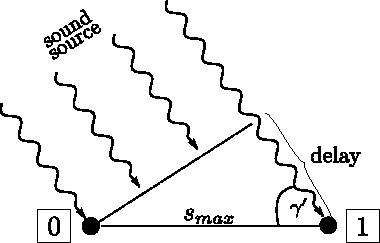
\includegraphics[width=0.4\columnwidth]{figures/tdoa_waves}
	\caption{Illustration of TDOA principle.}
    \label{fig:02_tdoa}
\end{figure}
% -------------------------------------------------------------

Specifying the speed of sound $c_s$ being 343\si{m/s} in air, the angle
$\gamma'$ can be defined as
\bsub \bal
    \gamma' &= cos^{-1}(\frac{|delay|}{s_{max}})
    \label{eq:02_tdoaAngle}\\
    \intertext{with}
    s_{max} &= \frac{f_s * d_{max}}{c_s}
\eal \esub
where $f_s$is the sampling rate.
% -------------------------------------------------------------

With the definition of a whistle signal as stated in \cref{eq:02_whistleSignal},
the microphone sensors $mic_1$ and $mic_2$ will output
\bsub \bal
    x_1(t) &= s(t) + n_1(t)\\
    x_2(t) &= \alpha s(t - D) + n_2(t).
\eal \esub
\label{eq:02_signalTimeDomain}
Here, $D$ is the delay of $x_2$ relative to $x_1$ for which is looked for.
\section{Cross Correlation}
\label{sec:02_cc}

The \ac{CC} provides information about the similarity of two signals.
Thus, the delay of one signal can be detected where the \ac{CC} function $R_{x_0x_1}(t)$ is largest.
% -------------------------------------------------------------
In time domain, the \ac{CC} of two signals $x_0$ and $x_1$ is denoted as
\bal
    R_{x_0x_1}(t) = \int^{+\infty}_{-\infty}x_0(\tau-t)x_1(\tau)d\tau.
\eal
Considering the frequency domain, the function can be transformed into
\bal
    \mathcal{F}[R_{x_0x_1}(t)] = G_{x_0x_1}(f) = X_0^*(f)X_1(f)
    \label{eq:02_ccBaseFunction}
\eal
with $\mathcal{F}[x_i(t)] = X_i(f)$ and $X_i^*(f)$ indicating the conjugate complex form.
% -------------------------------------------------------------
However, the finite observation time of the received signal corrupts the fourier
transform \cite{K_C_GCC}
and noise of sensors may introduce false peaks in the \ac{CC} \cite{H_B_GCC}.
% -------------------------------------------------------------
In frequency domain, the signals $x_0(t)$ and $x_1(t)$ from \cref{eq:02_signalTimeDomain}
can be expressed as
\bsub
\label{eq:02_signalFreqDomain}
\bal
    X_0(f) &= S(f) + N_0(f)\\
    X_1(f) &= \alpha S(f) e^{-j2\pi fD}+ N_1(f).
\eal \esub
% -------------------------------------------------------------
Thus, the \ac{CC} is
\bsub
\label{eq:02_Gx0x1}
\bal
    G_{x_0x_1}(f) &= \alpha |S(f)|^2 e^{-j2\pi fD} + N_0^*(f)N_1(f) + S^*(f) N_1(f) + \alpha S(f) e^{-j2\pi fD}N_0^*(f)\\
\intertext{which will be shortened as}
    G_{x_0x_1}(f) &= \alpha \phi_s(f) e^{-j2\pi fD} + \phi_n(f) + \phi_c(f) \label{eq_02_Gx0x1_simple} \\
\intertext{where}
\phi_s(f) &= |S(f)|^2 \label{eq:02_phi_s} \\
\phi_n(f) &= N_0^*(f)N_1(f) \label{eq:02_phi_n1n2} \\
\phi_c(f) &= S^*(f) N_1(f)+\alpha S(f)e^{-j2\pi fD}N_0^*(f) \label{eq:02_phi_c}.
\eal \esub
%\cite{H_B_GCC}
% -------------------------------------------------------------
Considering the ideal case where $s(t)$, $n_0(t)$ and $n_1(t)$ are uncorrelated, the terms
$\phi_c$ and $\phi_n$ disappear and the \ac{CC} results in
\bal
    R_{x_0x_1}(t) = \mathcal{F}^{-1}[\alpha \phi_s(f) e^{-j2\pi fD}] = \alpha \mathcal{F}^{-1}[\phi_s(f)] * \delta(t-D).
    \label{eq:02_R12_noNoise}
\eal
In general, $\phi_c$ and $\phi_n$ can neither be neglected nor assumed as uncorrelated to the signal \cite{H_B_prob},
so that they introduce inaccuracies and errors.

% -------------------------------------------------------------
% \unsure[]{do I fully understand this? Is this correct?}
% This means there exists a peak at delay $D$ which is altered by the \ac{iFT}
% of the signal spectrum.
As introduced, the \ac{CC} gives insight about the similarity of two signals and at peak, they
are most alike.
Received signals from microphone sensors are digital signals sampled with a certain
frequency.
The derivations are just as applicable, but transformations into frequency
domain are done by \ac{DFT}.
In the case of real data samples with length $n$ and similar \ac{DFT} size, the shift between
the zero index and the peak is the resulting delay $D$.
Zero index is defined as the index of the peak if no shift exists.
% -------------------------------------------------------------

\Cref{fig:03_ccTheory} is the outcome of two similar, but shifted sine signals with
3\si{\kilo\hertz} and normally distributed noise.
As the second signal is delayed by 10 samples, the peak can be detected where $shift = 10$.
The example signals are attached in \cref{fig:ap1_signals}.
One disadvantage of this technique is that for periodic signals the \ac{CC} also is periodic
and the peak is not always easily detectable. Noise and inaccuracies of the \ac{FFT} then
may influence the result what can make the peak unobvious \cite{L_L_GCC}.
\begin{figure}[ht]
	\centering
		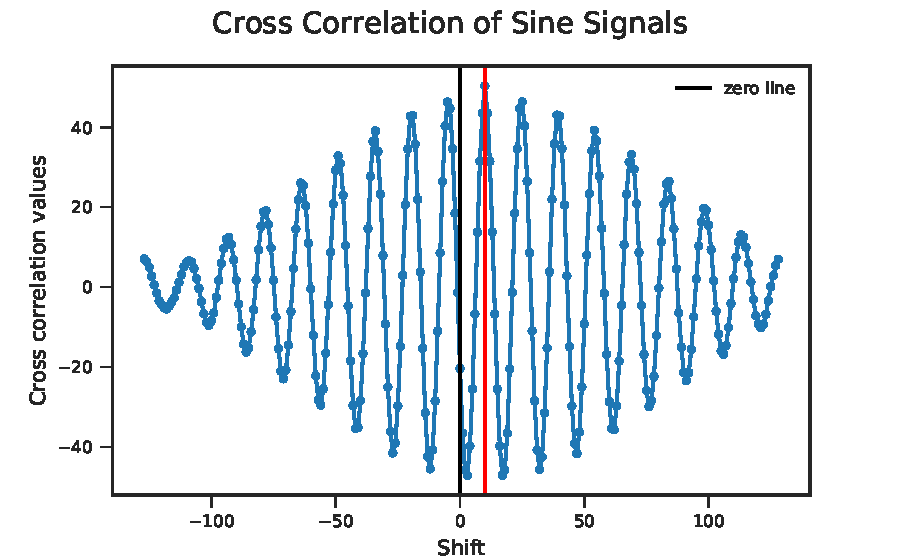
\includegraphics[width=1\columnwidth]{figures/CC_theory}
	\caption{Cross correlation of two generated sine signals with 3\si{\kilo\hertz}.}
    \label{fig:03_ccTheory}
\end{figure}

\section{Generalized Cross Correlation}
The generalized cross correlation is super duper nice.

\section{Signal Start Detection}
\label{sec:02_signalStartDetection}

One focus of the whistle signal localization is the correct choice of the
signal frame, with which the \ac{TDOA} measurement is done.
In order to perform the \ac{FFT} most efficiently, the size of one frame
should be a power of 2.
Assuming that the clearest signal without reverberation and with minimal
multipath propagated subsignals is at the start of a sound signal,
the frame to investigate is chosen to be at the beginning of a whistle sound.
Several methods exist and can be combined at will.
In the next subsections, signal start detection using entropy, energy and
zero crossing rate are subject of discussion.

\subsection{Entropy}
%\section{Signal Phase Difference}
\label{sec:02_phase}

With a different approach to the correlation methods, the \ac{TDOA} can be
detected by observing the phase of one reference frequency $f_c$.
Imaging a single-sinusoidal signal moving from left to right as
pictured in \cref{fig:02_phaseTheory}, two distant sensors
(\textit{channel 2} and \textit{channel 3}) will
receive different parts of the signal at the same time.
Transforming the frames into frequency domain by \ac{FFT}, the pase of the
maximal frequency differ by the delay.
% -------------------------------------------------------------

\begin{figure}[ht]
	\centering
		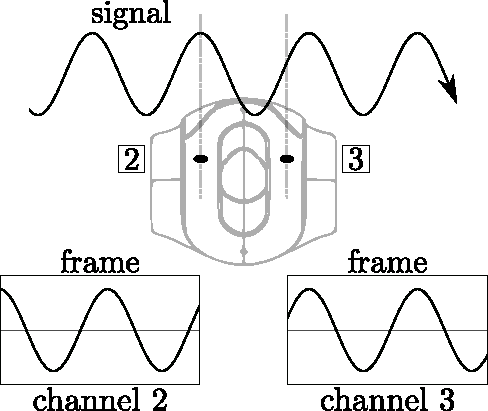
\includegraphics[width=0.35\columnwidth]{figures/phase_theory}
	\caption{Explanatory illustration of the phase difference method.}
    \label{fig:02_phaseTheory}
\end{figure}
% -------------------------------------------------------------

The phase of a signal's reference frequency is easily computable in frequency domain
with
\bal
    \phi(f_c) &= tan^{-1}\left(\frac{imag(X(f_c))}{real(X(f_c))}\right).
\eal
% -------------------------------------------------------------
With the difference of the phases of two channel, the delay in meters is defined as
\bal
    D &= \frac{\Delta \phi \cdot c_s}{2 \pi \cdot f_c}.
\eal
From that, the direction angle calculation of \cref{eq:02_tdoaAngle} can
be followed.
It should be noted that certain requirements needs to be fulfilled to receive a
unambiguous result due to signal periodicity.
\Cref{subsubsec:03_phase} covers the conditions that apply for this thesis's
hardware.
% -------------------------------------------------------------
%\input{content/02_Trigonometry}
\section{Front and Rear Distance}
\label{sec:02_distance}

For simplicity, the direction of the sound source is determined in
horizontal plane only.
However, the front and rear microphones differ 0.0212\si{m} in height
what can provide rough information about the distance of the sound source
for the particular case when the signal comes straight from front or behind.
If $delay_{01}$ and $delay_{32}$ are both very small, the signal comes from
the front or the back most likely.
Figure ...\missing[]{reference to nao channel figure} evinces, that one of
the sidewise delays need to be larger or equal to 5.41 \change[]{number to variable?}
samples for a signal to arrive from sideways.
When the delays of the side channels are smaller, they can be used to
detect the angle of the sound source in vertical YZ plane.

Figure \cref{fig:02_headSideTdoa} is a lateral illustration of
the Nao's right microphones $channel_1$ and $channel_3$.
% -------------------------------------------------------------
\begin{figure}[ht]
	\centering
		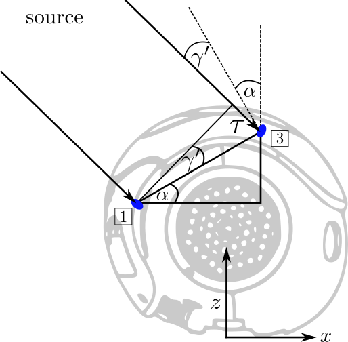
\includegraphics[width=0.45\columnwidth]{figures/side_head_tdoa}
	\caption{}
    \label{fig:02_headSideTdoa}
\end{figure}
% -------------------------------------------------------------
With the delay samples $\tau$, the angle of the sound source $\gamma$ relative
to the Z-axis can be determined with
% -------------------------------------------------------------
\bsub \bal
\gamma &= \alpha + \gamma'\\
\gamma' &= sign(delay) \cdot sin^{-1}(\frac{delay}{samples_{max}})\\
\intertext{with}
\alpha &= tan^{-1}(\frac{\Delta z_{channel}}{\Delta x_{channel}})
\eal \esub
which is the angle to the orthogonal axis to the plane though
front and rear channels.
% -------------------------------------------------------------
\begin{figure}[ht]
	\centering
		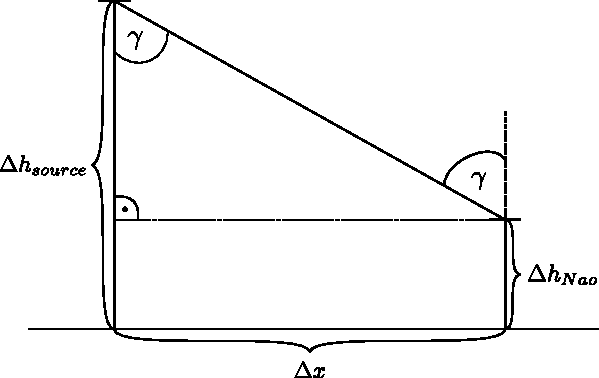
\includegraphics[width=0.6\columnwidth]{figures/x_distance}
	\caption{}
    \label{fig:02_xDistance}
\end{figure}
% -------------------------------------------------------------
Known that the sound source is positioned above of the robot, the distance
of the sound source can be approximated with an assumed height $\Delta h_{source}$
of the source.
So, the distance to the sound source is
% -------------------------------------------------------------
\bal
\Delta x &= (\Delta h_{source} - \Delta h_{Nao}) \cdot \tan(\gamma).
\label{eq:02_deltaX}
\eal
% -------------------------------------------------------------

%\input{content/02_filter}


\cleardoublepage
\chapter{Implementation}

\missing[inline]{
    * Alsa\\
    * Where in HULKs code and general HULKs framework\\
    * How WhistleLocalization is implemented\\
    * How TeamWhistleLocalization is implemented\\
    * CC Implementation\\
    * GCC Implementation\\
    * Phase Diff Implementation\\
}

\subsection{Signal Start Detection}
\label{subsec:03_signalStartDetection}

As mentioned in \cref{sec:02_signalStartDetection}, the detection of the
signal start is crucial for the localization.
The implementation of the different approaches will be presented coupled with
an examination of real measurement data.
To reduce undesirable effects and demonstrate the simplest form, a sinusoidal
signal of $3\si{\kilo\hertz}$ was recorded with the same circumstances as the
whistle sounds.
For the following data, the sound source was placed $2\si{m}$ in front of the robot.
In order to find the time point where the signal starts, information about
smaller fractions are required.
So, the original $44100$ samples that were buffered by the
\lstinline!WhistleLocalization! module are divided into several overlapping
frames with size $256$. The computational effort raises with smaller frame size,
but delivers a higher precision in return.
In order to perform the \ac{FFT} most efficiently, the size of one frame
should be a power of 2.
To compute the energy and entropy, the frames are transformed into
frequency domain with the \ac{FFT}.
The \ac{ZCR} does not require such a transformation.
In the evaluation \cref{sec:04_signalStartDetection}, the result of the single
methods are compared to each other.
For better visualization, the following data is shortened to $2400$ samples.

\missing[]{Start detection by frequency, whistle detection}

\subsubsection*{Spectral Entropy}

The formula to calculate the spectral entropy of a signal is introduced as
\cref{eq:02_entropy} in the previous chapter.
For the entropy information, the signal must not be cleaned previously.
By looking at the derivation of the entropy, a global minimum can be found
at the starting point of the signal due to its change from noise to signal.
The starting index is therefore defined by the index of the derivation's minimum.
Of course, this approach does not work real-time but with small delay.
\Cref{fig:03_entropy} is a plot of the recorded sine signal with the corresponding
entropy.
According to the frame size, the accuracy of the start index can be increased.
However, the frame size is limited by the required number of samples for one \ac{FFT} and
its computational effort.
% -------------------------------------------------------------
\begin{figure}[ht]
	\centering
		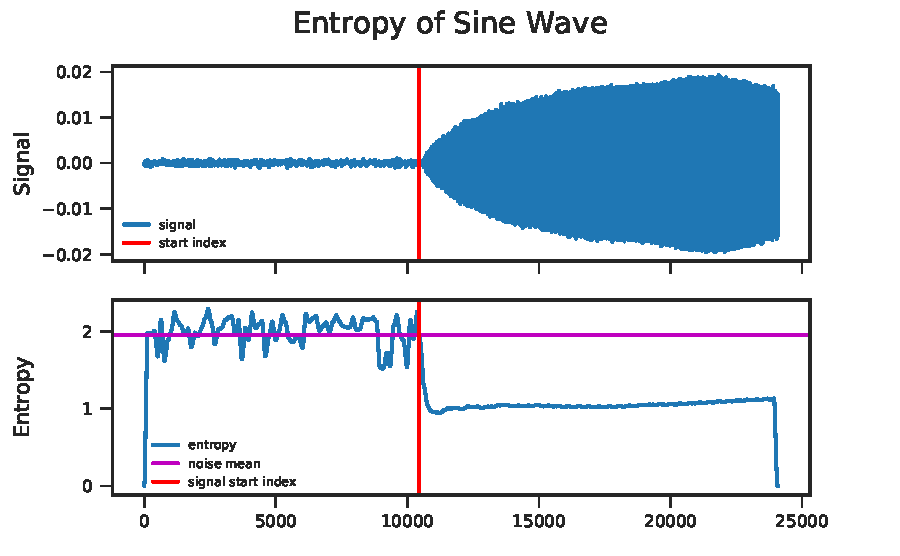
\includegraphics[]{figures/sine_entropy}
	\caption{Exemplary entropy of a sinusoidal signal with 3\si{\kilo\hertz}.}
	\label{fig:03_entropy}
\end{figure}
% -------------------------------------------------------------
In \cref{subsec:04_entropy}, the entropy outcome of a whistle sound
and its derivation is presented for evaluation.

\subsubsection*{Energy}

As mentioned above, the total signal is divided into multiple overlapping frames.
\Cref{eq:02_spectralEnergy} represents the energy of each frequency
component.
According to this, the energy of one of those frames is \cref{eq:02_energy}.
Assuming that the energy holds for the whole frame, overlapping and adding the energy
results in \cref{fig:03_energy}.
If the frequency of the examined signal is known as for the whistle, only energy values
of the relevant frequencies needs to be considered.
One downside of the energy information is that the threshold has to be adapted
manually for the related environment.
Especially at the tournament, parameters like these should be avoided and thus,
the start detection by energy is inconvenient.
% -------------------------------------------------------------
\begin{figure}[ht]
	\centering
		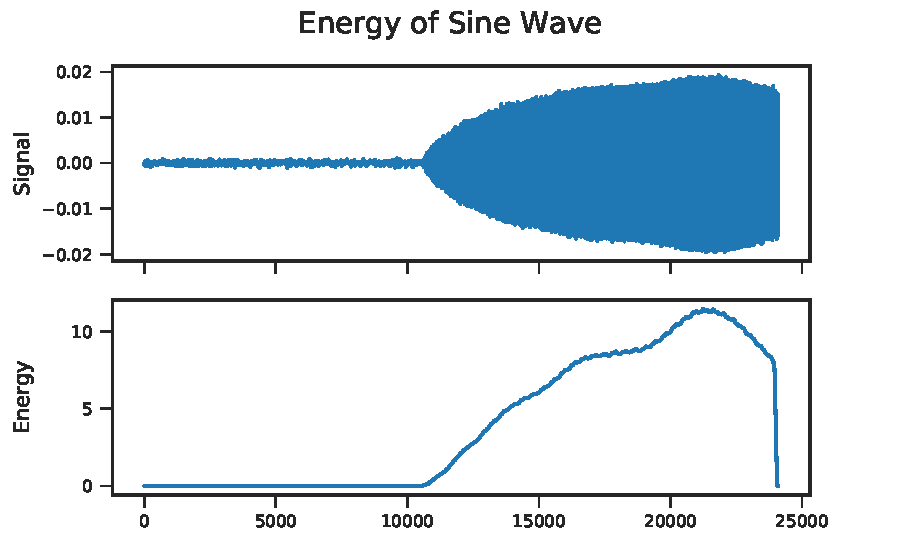
\includegraphics[]{figures/sine_energy}
	\caption{Energy of a sinusoidal signal with 3\si{\kilo\hertz}.}
	\label{fig:03_energy}
\end{figure}
% -------------------------------------------------------------

\subsubsection*{Zero Crossing Rate}

Alike the other methods, the buffered signal is divided into smaller frames
which can be set arbirary small for the \ac{ZCR} where no \ac{FFT} is necessary.
% To receive a higher accuracy, the frames of the \ac{ZCR} can be set small.
% are set to 80 samples.
In each frame, the sign changes are counted which only requires simple implementation
and computationally lightweight.
It is known that only noise is received at the beginning of the measurement and on the
contrary, signal noise is present at the end.
By comparing the mean of the received noise at the beginning of the measurement and
the mean of the signal part, a dynamic threshold can be defined and the beginning of the
signal is detectable.
In this work, the crossing of the threshold is observed from the last
value to the first.
Number of noise and signal frames are parameter values which depend
on the amount of samples and the size of the frame.
% In \cref{fig:03_zcr} and in this work, the threshold is set by multiplying the
% mean of the noise and signal mean by factor 1,25.
\begin{figure}[ht]
	\centering
		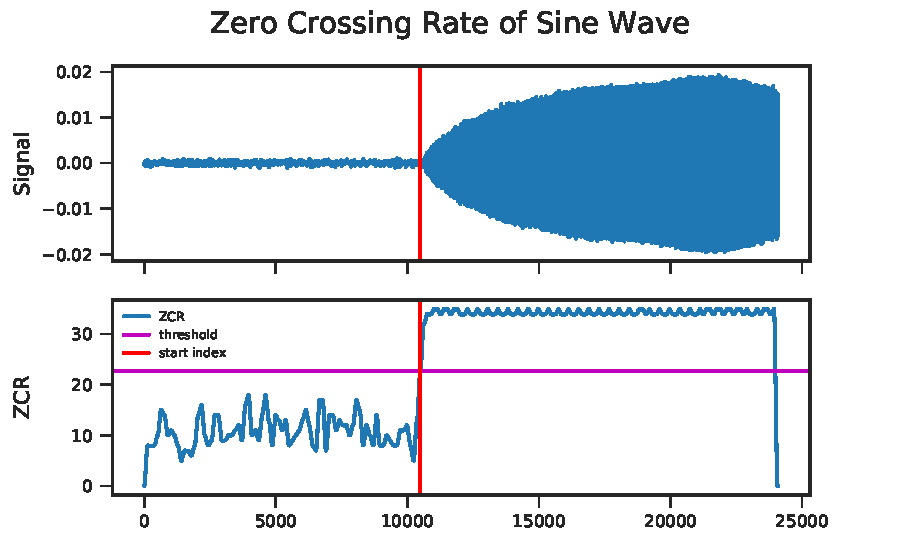
\includegraphics[]{figures/sine_zcr}
	\caption{Zero Crossing Rate of a sinusoidal signal with 3\si{\kilo\hertz}.}
	\label{fig:03_zcr}
\end{figure}
According to the circumstances, the threshold can be lowered optionally.
For real whistle data, the mean of noise and signal mean is reduced by factor 0,9 to
lower the threshold and results are shown in \cref{subsec:04_zcr}.


\cleardoublepage
\chapter{Evaluation}

\section{Signal Start Detection}
\label{sec:04_signalStartDetection}

\todo[inline]{This section seems a bit misplaced. I feel like "Team Evaluation"
should be the last evaluation section. Is there a reason why you can't put this
before that?}

In previous chapters, the importance of the signal start was emphasized.
% Due to the fact that the direction detection methods is
% executed on smaller frames than the actual whistle detection.
% To demonstrate this for the phase method, the frame to examine is
% shifted with time \cref{subsec:04_frameNumber}.
Especially the result in \cref{subsec:03_phase} has shown that in fact, the
accuracy of the direction predictor decreases when evaluated on later samples
of the whistle signal.\todo{Maybe interpret this somewhere: give a reason
why shit makes sense (e.g. maybe because more reflections of the signal will
have reached the microphone)}
Also according to the outcome of \cref{subsec:04_psnr}, the \ac{GCC}
method performs best with frames near to the signal start. \todo[inline]{Get
rid of some cross-references and/or write more about what happened in these
chapters. (I don't remember what happened in 3.4 and 4.2.3 and jumping back and
forth is annoying.)}

% There are some reasons why other methods were tested to find the signal start.
In order to find a good solution for a highly reliable, accurate but
computationally tractable start detection, different approaches were
tested profoundly.
For high temporal\todo{I added "temporal" here because otherwise it seems unintuitive
that a less samples is better (because at the same time it might be harder to
predict from fewer samples as there is less information in the frame)} accuracy
either the number of samples in a frame have to be small\todo{Maybe rather say
that the frame as to be small? A low number of samples in a frame could also be
achieved by a smaller sampling rate, which would not help.} or the window must
be shifted with small steps which both implicit a large number of evaluations.
The existing whistle detection algorithm of the HULKs presented in
\cref{subsec:03_whistleDetection} is computationally intensive and has a low
accuracy for small frames\todo{Is "frames" actually the correct term (in
general)? Shouldn't it be "window"? I don't know what people use in signal
processing literature} as shown in \label{subsec:04_whistleDetection}.
Therefore, the goal is to identify a\todo{"looked" doesn't work this way. You are using this
quite a lot. Maybe grep the document for it and replace it.} simple algorithm for
the signal start detection. Ideally, this algorithm should be adaptable to
signals other than the whistle sounds.\todo{I would add a reference to the section
where you presented these algorithms. (this is only the evaluation, right?)}

Hereinafter, the performance of each method methods is evaluated by
analyzing the error between algorithmically determined start index
and manually labelled start index.
As a benchmark, the prediction accuracy is evaluated on 11 measurements on all
robots\todo{how many robots?} \todo{this sentence is missing some
words}\cref{subsec:04_labMeasurements}.
By the frame size of the \ac{FFT} being set to 256 samples for the
correlation methods, a start index error of at most 256 samples is
desired.
Therefore, a start index detection result is regarded as failure for errors
larger than 256 for the following sections.
Two metrics are specified to express the degree of failure.
The former counts the number of large errors for each channel.
In this case, 220 sample data for 11 measurements on five robots with
four channels each exist.\todo{I don't understand this sentence.}
The second metric reports the number of measurements for which any of the
channels failed. For this case, 55 measurements are given.\todo{Again, what is
this sentence saying? I thought we had 11 measurements? Or is it 11
measurements * 5 robots? Maybe simply write 55 in the first place (rather than
11)}.
% -----------------------------------------------------------------------------------------------------

\subsection{Whistle Detection}
\label{subsec:04_whistleDetection}

\todo[inline]{It is not immediately clear that with "whistle detection" you refer
to the "whistle detection of the HULKs", e.g. your "baseline"}
First, the accuracy of the whistle detection in regard of the start index
is evaluated.
Here, the start index is defined as the first index where the whistle detection
found a whistle.
With a frame size of 1024, the whistle detection algorithm fails in every of the
55 measurements with at least one channel if only an error of at most 256 samples
is permitted.
However, every error is in the range of 1024 samples which proves that the
approximate start of the whistle sound is detected correctly.
With a smaller frame size of 256, the temporal accuracy is improved but
introduces false positive detections.\todo{do you have numerical results here?}
With the results, one can say that the whistle detection is not sufficient
for the start detection or is at least not reliable as stand-alone solution.
Furthermore, this approach is limited to sounds in fixed and known frequency range.
%  failure rate of
% 9\si{\percent} in regard to every channel.
% In this work microphone data were saved as soon as the whistle detection module
% found a whistle sound in the audio samples.
% Due to this implementation, the algorithm does never fail to detect the whistle
% Standing alone, the error is always in the range of \si{\pm1024} samples due to the
% set frame size of 1024 samples.
% With a smaller frame size of 256, the accuracy gets better with an error of
% 9\si{\percent} in regard to the 220 sample data but has an error rate of
% 25,5\si{\percent} for the measurements.

% looking at the next 300
% values and with a step size of 50 the result is 15\si{\percent} and 36\si{\percent}
% and with step size 1, it is 13\si{\percent} and 33\si{\percent}.
% This is computationally very costly and the reward is small.

\subsection{ZCR}
\label{subsec:04_zcr}

For the evaluation of the \ac{ZCR},
the frame size is set to 256 samples and number of noise and signal frames
are set to 10 frames.
In 7\si{\percent} of the 220 channel sample data\todo{"sample data" sounds like
it is not a term. Maybe only "samples"?}, the method fails with a significant
error larger than 256 samples.\todo{I don't thing you have to repeat the 256
sample criterion every time. You defined what is considered a failure earlier.
Just say "failed".} In most cases, the method provides accurate results with
small error. Taking all measurements of robot 26 as example, the \ac{RMSE}
amounts 54.23 samples.\todo{Again, where is the data for this? Tables, figures?}

However, there are cases where the algorithm fails. Looking at those cases it
could be identified that the errors occur often due to incorrect assumptions
that the signal is present at the end of the buffered samples.
Some measurements prove that this is not always the case as shown in
\cref{fig:04_zcrFail}.
Here, the data of the front right channel of robot 21 with the whistle source
at position 5 in \cref{subsec:04_labMeasurements}
illustrates how the signal ended around 35000 samples already. \todo{Neither
the robot number, nor the position or the channel are relevant here I think.}
If the start index is determined at the point where the \ac{ZCR}
falls below the threshold searching backwards as stated in \cref{sec:02_signalStartDetection},
the detection fails.

In most cases, only one out of four channels produces a erroneous
result.\todo{Why? Doesn't the signal end early on all channels?}
Because the final start index on one robot is set equal for all channel,
the failure can be compensated with a simple voting procedure.
% -------------------------------------------------------------
\begin{figure}[ht]
	\centering
	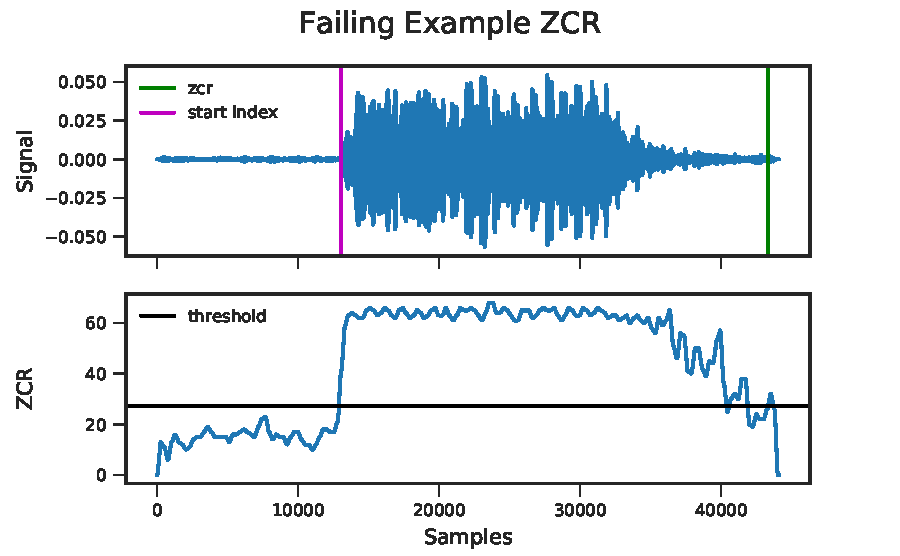
\includegraphics[]{figures/evaluation/zcr_fail}
	\caption{Channel 3 data from measurement 5 of \cref{subsec:04_labMeasurements}
		for robot number 21. A failing example for the start detection by \ac{ZCR}
		is shown.}
	\label{fig:04_zcrFail}
\end{figure}
% -------------------------------------------------------------
If the start index is determined at the point where the \ac{ZCR}
falls below the threshold searching backwards as stated in \cref{sec:02_signalStartDetection},
the detection fails.

In most cases, only one channel of four output a erroneous result.
Because the final start index on one robot is set equal for all channel,
the failure can be compensated with a smart voting procedure.

Another option exists by changing the process of finding the
threshold excess onwards.\todo{I don't understand what this is saying.}
In this case, the threshold is scaled with a factor of 1.25.
Results by this were poorer than the initially implemented manner
with a failure rate of 15\si{\percent}.\todo{Did you ever report the previous failure rate?}
By adding the constraint that multiple samples must exceed the
threshold successively, result can be slightly improved for the cost of higher
computational effort.

It should be noted that the poor performance of the \ac{ZCR} method with signal that
was cleaned with spectral subtraction previously. This surprising outcome is
convenient for the overall task, because the start index result can be embed
into the spectral subtraction, providing information for separating the noise
and signal part.\todo{I don't get what this paragraph is saying?}

\subsection{Entropy}
\label{subsec:04_entropy}

As discussed in \cref{subsec:02_Entropy} the entropy quantifies the amount
of chaos in a signal frame.\todo{Is this correct? Chaos is deterministic and not
the same as randomness}
Especially for signals to localize with unknown characteristics,
this method can be useful because no a-priori knowledge is needed.\todo{You should
probably say that the only prior knowledge must be, that the signal to detect
has lower entropy than the background noise.}
For all measurements this method yielded poorer results than the \ac{ZCR} method
with a failure rate of around 20\si{\percent}.
Best results are achieved with a frame size of 512 samples and a step size of 800
samples.
% \change[]{Explain what steps are? Maybe in implementation?}
However, for records with fading whistle the entropy method
generates more reliable results than the \ac{ZCR} method.\todo{What do you mean
by "fading whiste"? Whistles that don't have a distinct/abrupt start?}
Taking the same measurement as an example for which failure of the \ac{ZCR} method
was discussed earlier, \cref{fig:04_entropyGood} shows how the algorithm
detects the signal start correctly even though the whistle sound ended at
around 35000 samples. In this measurement, the start index errors of all four
channels were smaller than 40 samples.
% -------------------------------------------------------------
\begin{figure}[ht]
	\centering
	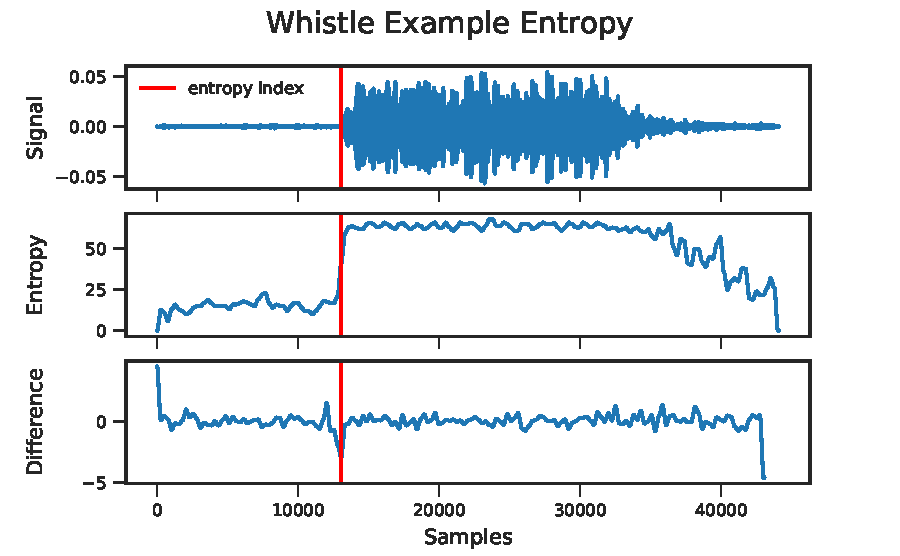
\includegraphics[]{figures/evaluation/entropy_good}
	\caption{Exemplary result of start index detection by entropy where
			the \ac{ZCR} method failed due to fading whistle
			at the data.}
	\label{fig:04_entropyGood}
\end{figure}
% -------------------------------------------------------------

% But as the entropy should be larger for noisy environment
% performance in other surrounding of measurement at \ac{RoboCup} is looked at.
% Entropy would be best for undefined signal -> distinguish between
% signal and noise without information

\section{\acl{WSDE}}
\label{sec:04_tdoaSingle}

Before evaluating the performance of the different methods as a whole,
% For comparability of the results,
one exemplary measurement is utilized
to present and analyse the \ac{TDOA} methods in detail first.
In this recording, the sound source is placed at the right front
of the robot with 4.5\si{m} distance.
Hereinafter, this measurement will be referenced to as \textit{demonstration-dataset}.
This corresponds to an an angle of -33.7\si{\degree} in robot coordinates.
To get an idea about the examined data, according whistle signal samples around the
start are plotted in \cref{fig:04_tdoaSignal} for all channels.
% -------------------------------------------------------------
\begin{figure}[ht]
	\centering
		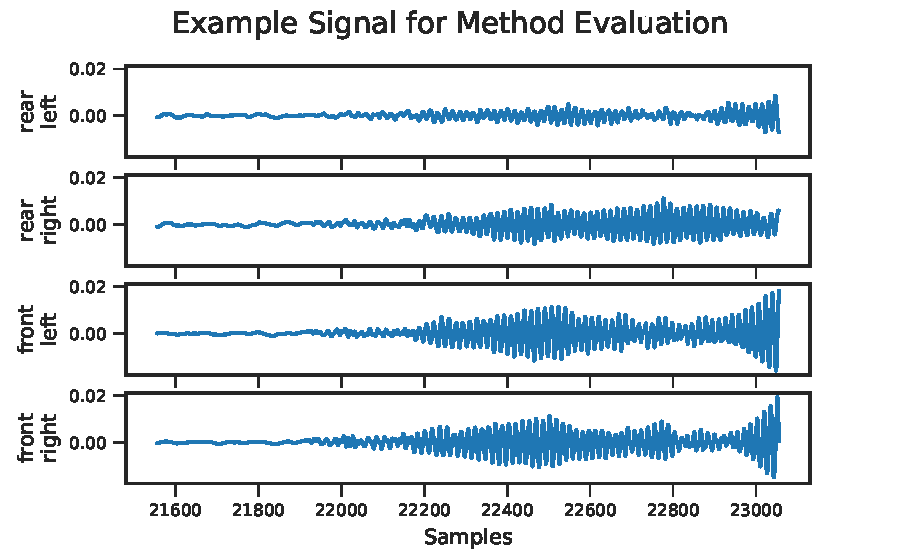
\includegraphics[]{figures/evaluation/cc_frontRight_1_signal}
	\caption{Signal start section of a whistle sound recorded from front right.}
	\label{fig:04_tdoaSignal}
\end{figure}
% -------------------------------------------------------------

As the next sections focus on the performance of the \ac{TDOA} methods,
the start index is set manually.

For the sake of conciseness, throughout the following sections the correlation
function $R_{x_ax_b}$ of two signals $x_a$ and $x_b$  (\cf
\cref{chap:02_prerequisites}) is denoted as $R_{ab}$.


\subsection{Cross Correlation}
\label{subsec:04_ccSingle}
% -------------------------------------------------------------

The \ac{CC} is a widespread technique to obtain the time delay
between two series of samples.
To discuss the result of the \ac{CC}, the belonging correlation functions
of the demonstration-dataset are plotted in \cref{fig:04_cc}.
The selection process and implementation correspond to the explanations
in \cref{subsubsec:03_cc}.
For $R_{32}$ and $R_{13}$ a peak is clearly visible.
However, for the other \ac{CC} the problem of a weak peak
arises what was mentioned as downside of the \ac{CC} in \cref{sec:02_cc}.
% -------------------------------------------------------------
\begin{figure}[ht]
	\centering
		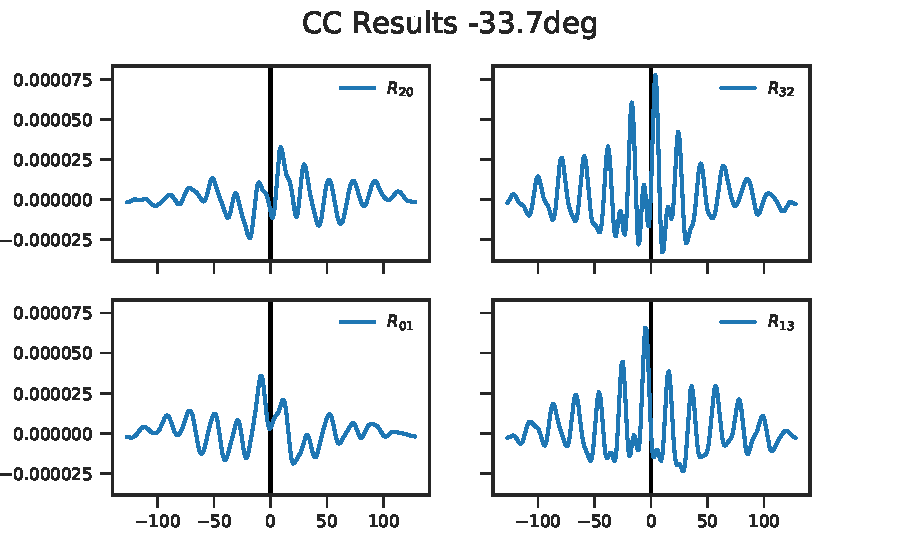
\includegraphics[]{figures/evaluation/cc_frontRight_1}
	\caption{Cross correlation results of signal from front right (-33.7\si{\degree}).}
	\label{fig:04_cc}
\end{figure}
% -------------------------------------------------------------
\btline{ht}{1.2}
\btab{|c|c|c|c|c|}
\hline
Base Channel & Next Channel & Delay & Candidate (-) & Candidate (+)\\
\hline
0 & 1 & -8.25 & -144.9 & -35.1\\
\hline
1 & 3 & -4.59 & -17.4 & 78.6\\
\hline
2 & 0 & 9.16 & -30.6 & -30.6\\
\hline
3 & 2 & 3.94 & -150.2 & -29.8\\
\hline
\etab
\et{Cross correlation delay results of signal from front right}{04_cc}
% -------------------------------------------------------------

According to the delays in \cref{tab:04_cc}, two source direction candidates arise
for each channel pair.
By the implementation in \cref{subsec:03_directionCandidates}, the combination of
all options with the smallest error is selected as \ac{WSDE}.
Hence, the algorithm outputs -26.9\si{\degree} what produces an error of 6.8\si{\degree}.
The delay between channel 2 and 0 is larger than the maximum delay of 6.85 samples
and therefore cut to the maximum sample delay.
Besides these, the \ac{TDOA} between the channel pairs produce one appropriate
direction candidate which correctly points to the sound source.
% -------------------------------------------------------------

\subsection{Generalized Cross Correlation}
\label{subsec:04_gccSingle}
% -------------------------------------------------------------
\Cref{fig:04_gcc} presents the \ac{GCC} result by the \ac{GCC-PHAT} method of
the demonstration-dataset equal to \cref{subsec:04_ccSingle}.
The subsample delays for each channel pair and their resulting direction candidates
are listed in \cref{tab:04_gcc}.
From this, a final direction of -30.0\si{\degree} is determined
resulting in an error of 3.69\si{\degree}.
It is apparent that the peaks of the \ac{GCC} are better to detect than the peaks of the
\ac{CC}.
% -------------------------------------------------------------
\begin{figure}[ht]
	\centering
		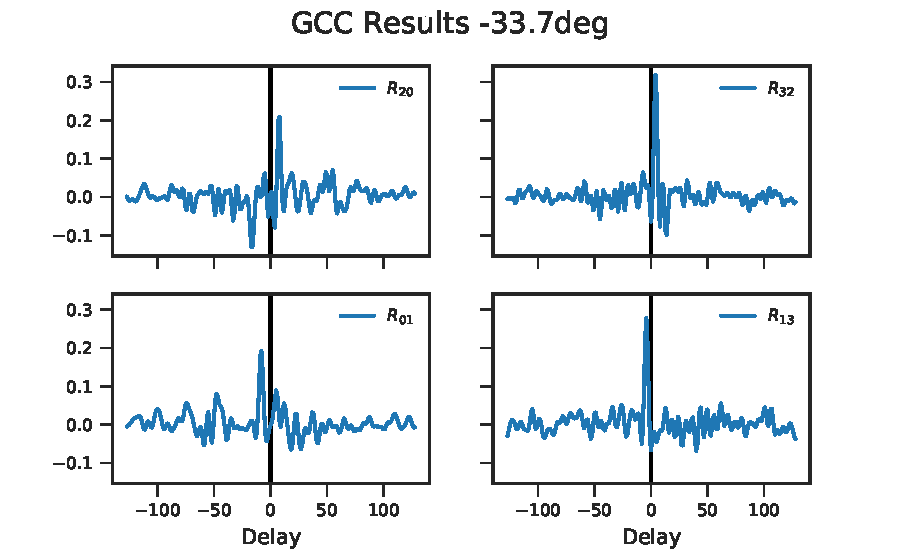
\includegraphics[]{figures/evaluation/gcc_frontRight}
	\caption{Generalized cross correlation results of signal from front right.}
	\label{fig:04_gcc}
\end{figure}
% -------------------------------------------------------------
\btline{ht}{1.2}
\btab{|c|c|c|c|c|}
\hline
Base Channel & Next Channel & Delay & Candidate (-) & Candidate (+)\\
\hline
0 & 1 & -8.28 & -144.7 & -35.3\\
\hline
1 & 3 & -4.09 & -22.8 & 84.0\\
\hline
2 & 0 & 7.60 & -30.6 & -30.6\\
\hline
3 & 2 & 4.13 & -148.7 & -31.3\\
\hline
\etab
\et{Generalized cross correlation delay results of signal from front right}{04_gcc}
% -------------------------------------------------------------
\subsection{Phase Difference}
\label{subsec:04_phaseSingle}

For detecting the source direction with phase difference, a smaller frame
size of 64 samples is defined.
In \cref{subsubsec:03_phase} two variants of this method were introduced that use
different strategies to identify a reference frequency. The first version uses
a static reference frequency that is fixed a-priori by the user. The second version
dynamically estimates a dominant frequency across all four channels. Hereafter,
the performance of both variants is discussed.


\subsubsection*{Static Reference Frequency}

In \cref{subsubsec:03_phase} two different ways to set a reference frequency $f_c$
for the phase difference method were introduced.
First, a suitable value for the reference frequency is specified by
examining the influence of the chosen value.
Therefore, \ac{WSDE} results with the phase difference method are evaluated by setting
different values for the reference frequency within whistle range.
For this purpose we consider all of eleven measurements of the the laboratory-dataset
recorded with robot no. 26 at the center point.

According to \cref{subsubsec:03_phase}, the most feasible frequency is defined as
2775.08\si{\hertz} by the distance between the channels
and the whistle spectrum ranges between 2\si{\kilo\hertz}
and 4\si{\kilo\hertz}.

As shown in \cref{fig:04_diffFc} shows, the \ac{RMSE} is high for
frequencies smaller than 2600\si{\hertz}.
With a frequency of 2024.12\si{\hertz}, error is largest.
% The result complies with the information in \cref{fig:03_maxFreq} showing that
% frequencies higher than 2500\si{\hertz} are dominant in whistle signals.
With this outcome, the fixed frequency is set to 2670.1\si{\hertz}
for further usage of the direction detection by phase method.
Limitation exists due to the ambiguity of the signal which is
content of \cref{subsubsec:03_phase}.
% -------------------------------------------------------------
\begin{figure}[ht]
	\centering
		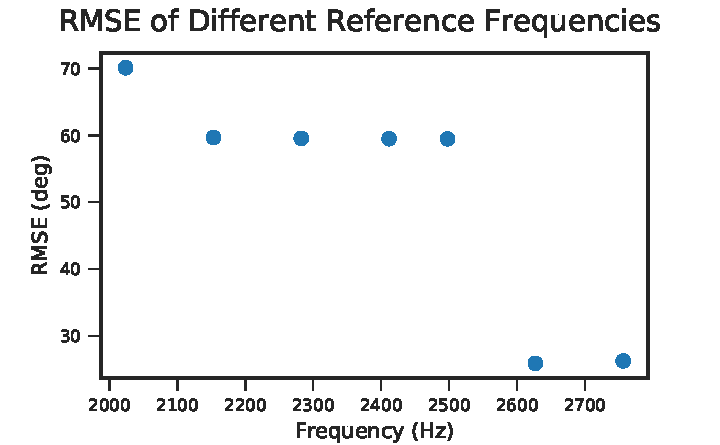
\includegraphics[]{figures/evaluation/phase_fc_rmse}
	\caption{Result of all measurements done with robot 26 to compare different
	fixed frequency values in whistle range.}
	\label{fig:04_diffFc}
\end{figure}
% -------------------------------------------------------------

On the basis of the results, the reference frequency was set to a minimum
of 2600\si{\hertz} for evaluation of the demonstration-dataset.
Hence, the reference frequency is 2627.1\si{\hertz} in the case of a \ac{FFT} length
of 256 samples.
Applying the phase difference method with this reference frequency, the final
direction estimate computed from the candidates listed in
\cref{tab:04_fixedFreqResult} is -29.6\si{\degree} which results in an error of
4.1\si{\degree}.
% -------------------------------------------------------------
\btline{ht}{1.2}
\btab{|c|c|c|c|c|}
\hline
Base Channel & Next Channel & Phase Difference & Candidate (-) & Candidate (+)\\
& & [\si{\deg}] & [\si{\deg}] & [\si{\deg}] \\
\hline
1 & 3 & -79.1 & -26.8 & 88.0\\
\hline
2 & 0 & 167.7 & -30.6 & -30.6\\
\hline
3 & 2 & 88.5 & -148.7 & -31.3\\
\hline
\etab
\et{Resulting candidates of phase difference method with fixed frequency
	2670.1Hz of example measurement from front right
	(-33.7\si{\degree})}{04_fixedFreqResult}
% -------------------------------------------------------------

\subsubsection*{Dynamic Reference Frequency Selection}

Another option is to have a nonspecific reference frequency that
is computed dynamically without a-priori knowledge.
As stated in the implementation chapter, frames are chosen where the frequencies
of the maximum amplitudes coincides for all channels.
For the running example discussed here, this corresponds to a frequency of 2756.25\si{\hertz}.

For comprehensibility, the determined frequency information visualized by
wave signals with the detected phases and amplitudes
in the lower subplot of \cref{fig:04_phaseSingle}.
In the upper plot of \cref{fig:04_phaseSingle} one sees the originally received microphone
data before applying a Hann window and transforming it into frequency domain by
\ac{FFT}. The resulting phases and amplitudes are listed in
\cref{tab:04_phaseSingle}.
% -------------------------------------------------------------
\begin{figure}[H]
	\centering
		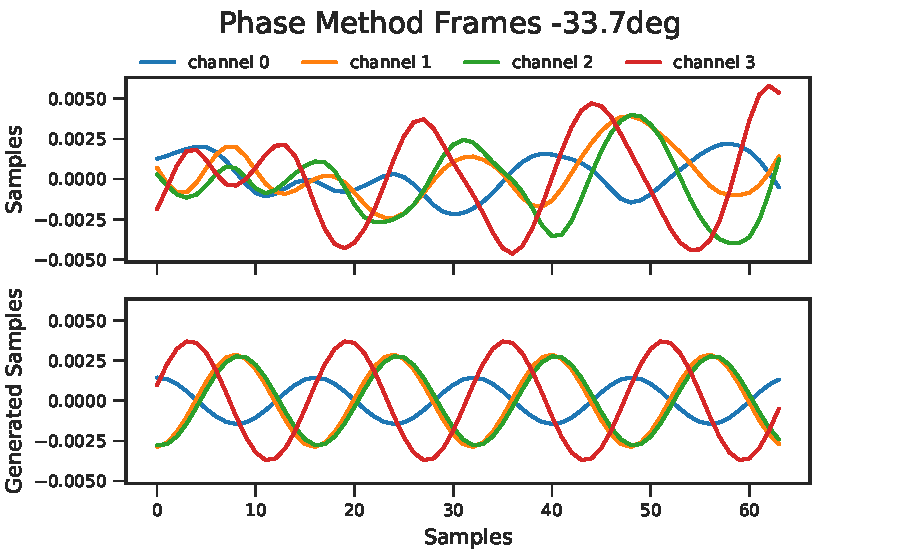
\includegraphics[]{figures/evaluation/phase_cos}
	\caption{Frames used for the direction detection by phase method.}
	\label{fig:04_phaseSingle}
\end{figure}
% -------------------------------------------------------------
\Cref{tab:03_maxFrequencies} pointed out that the most feasible frequency
of the rear channels 0 and 1 is not in whistle spectrum
due to the larger physical distance between the microphones.
Thus, the phase difference information is neglected because of the ambiguity of
the temporal sequence between the signals.
Following the procedure discussed in \cref{subsubsec:03_phase},
the resulting phase difference estimate
is -29.2\si{\degree} by combining the candidate direction -17.6\si{\degree},
-30.6\si{\degree} and -39.3\si{\degree} from channels 1, 2 and 3 according to
\cref{tab:04_phaseDiffSingle}.
% -------------------------------------------------------------
\btline{ht}{1.2}
\btab{|c|c|c|}
\hline
Channel & Phase [\si{\deg}] & Amplitude\\
\hline
0 & -1.55 & 0.00144\\
\hline
1 & -177.7 & 0.00287\\
\hline
2 & 173.4 & 0.00279\\
\hline
3 & -75.0 & 0.00372\\
\hline
\etab
\et{Phase and amplitude of frame signals with $f_c$ = 2756.25Hz}{04_phaseSingle}
% -------------------------------------------------------------
\btline{ht}{1.2}
\btab{|c|c|c|c|c|}
\hline
Base Channel & Next Channel & Phase Difference & Candidate (-) & Candidate (+)\\
& & [\si{\deg}] & [\si{\deg}] & [\si{\deg}] \\
\hline
1 & 3 & -102.7 & -17.6 & 78.8\\
\hline
2 & 0 & 173.4 & -30.6 & -30.6\\
\hline
3 & 2 & 113.1 & -140.7 & -39.3\\
\hline
\etab
\et{Phase differences and resulting direction candidates of demonstration-dataset
with dynamically determined reference frequency}
{04_phaseDiffSingle}
% -------------------------------------------------------------

\subsubsection*{Impact of Selected Frame}
\label{subsubsec:04_frameNumber}

Not only does the frequency play a major role for the phase method,
but also the samples chosen for analysis.
Again it is referred to the eleven measurements of the laboratory-dataset
recorded on the robot at the center point (no. 26).
To evaluate if and how the result changes over time, the selection window
is shifted by half the frame size from -5 shift steps to 20.
Recapitulating the implementation details for the static reference frequency case
in \cref{subsec:04_phaseSingle},
the first frame after the start index is chosen in which the whistle detection would
count a whistle signal.
This frame is represented by zero shift.

% [ 62.32629763  59.19634105  66.78950798  54.53898736  30.80692207
%   25.91537359  56.55427899  65.27548831  66.3898905   75.48670644
%   97.33965933  96.6373387  100.22012166 104.20160752  59.55737843
%   58.22148221  48.51237213  51.93254436  49.08273252  62.64453085
%   56.49506079  57.03430393  67.46509351  73.21671739  43.69704948]
In \cref{fig:04_phaseOverTime}, the resulting errors per shift
for all measurements are plotted, presenting the influence of the
selected frame around the signal start.
The reference frequency was set to 2627.1\si{\hertz} due to the
outcome that frequencies larger than 2600\si{\hertz} achieve best results.
The graph presents that frames nearest to the signal start reach best results
with an \ac{RMSE} of 25.9\si{\degree}.
These results show that the frame position has a significant influence on the prediction
accuracy of the direction detection.
Therefore, an accurate signal start detection is crucial for the preciseness of the \ac{SSL}
by phase difference.
% -------------------------------------------------------------
\begin{figure}[ht]
	\centering
		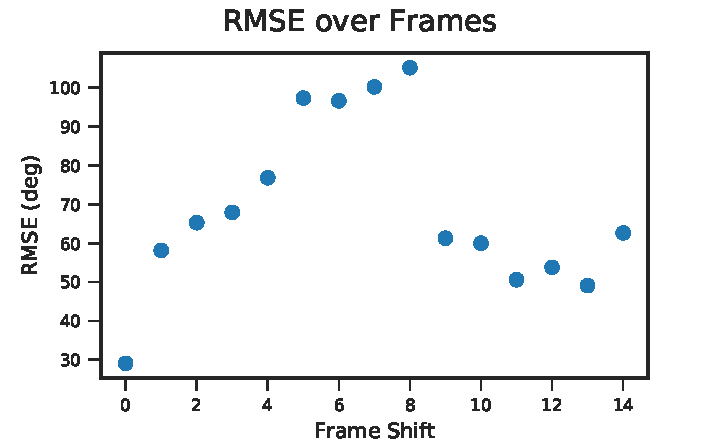
\includegraphics[]{figures/evaluation/phase_over_time}
	\caption{\ac{WSDE} result errors while shifting the frame over the
	samples of the laboratory-dataset on robot no 26.}
	\label{fig:04_phaseOverTime}
\end{figure}
% -------------------------------------------------------------

\subsubsection*{Phase Method Conclusion}
\label{subsubsec:04_phaseMethodConclusion}

Different options were investigated relating to the phase difference method
in the last subsections.
One finding is that reference frequency values should be chosen larger than
2.6\si{\kilo\hertz} for best results.
Another is that samples at the beginning of the signal are most suitable
for this method.
An advantage of the dynamically selected reference frequency is the reduction of
one parameter.
It requires more effort to implement and considering edge cases but
does not depend on the whistle detection.
Both approaches are valid for this work and result in a similar reference
frequency due to the limitations listed in \cref{subsubsec:03_phase}.

\subsection{\ac{TDOA} Method Comparison}
\label{subsec:04_singleRobotAngleError}

As the different \ac{TDOA} methods were discussed profoundly in the last
sections, all measurements of the laboratory-dataset are considered here
to make a generalized statement about the performance.
The \acp{WSDE} resulting from here are the inputs of the multi-agent
localization filter.
\Cref{fig:04_compareRmse} presents the \ac{RMSE} considering the
direction results of all five robots for each measurement in
\cref{subsec:04_labMeasurements}.
Additionally, the estimated standard deviation of each measurement
provides insight into the validity of the single robot results.
As one can see, the standard deviation of the relative angle of the \ac{GCC}
method is significantly smaller as compared to the phase method for most
measurements.
How this influences the reliability of the sound localization is
subject of discussion in \cref{sec:05_methodComparison}.
% -------------------------------------------------------------
\begin{figure}[h]
	\centering
		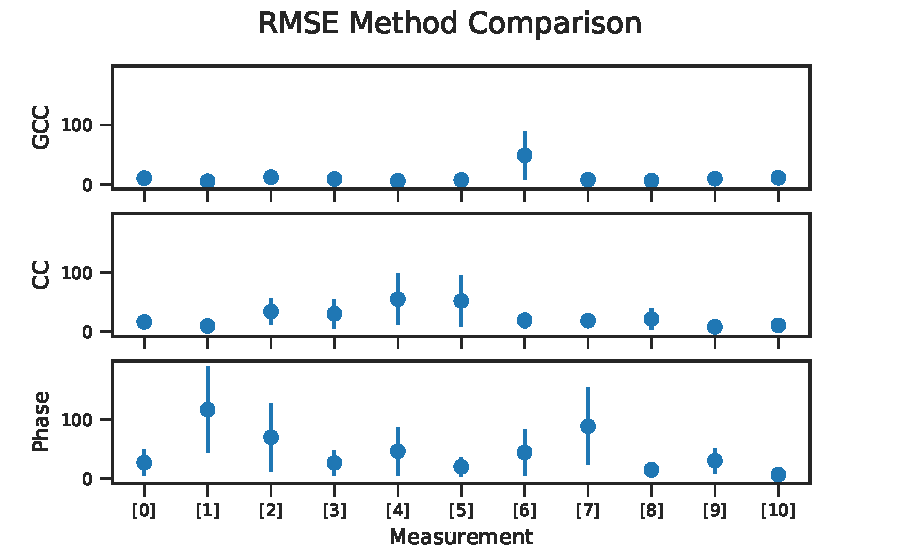
\includegraphics[]{figures/evaluation/compare_rmse}
	\caption{Angular RMSE and standard error of robot results per
	measurement of \cref{subsec:04_labMeasurements}.}
    \label{fig:04_compareRmse}
\end{figure}
% -------------------------------------------------------------

\subsection{Conclusion}
\label{subsec:04_tdoaConclusion}

The results in \Cref{subsec:04_singleRobotAngleError} show
that the \ac{GCC-PHAT} algorithm performs best according to the
laboratory-measurements.
Not only the errors are smallest, but also the low standard deviation
displays that the robots agree on the \ac{WSDE} and little outliers exist.
Also in regard to the multi-agent Bayesian updating filter, unified
results of the stand-alone robots are beneficial.
Another advantage of the \ac{GCC-PHAT} method is the presence of
a indication regarding the certainty of the measurement.
Interpreting the \ac{PSNR} as such, it can be used to detect outliers
or consider results with small \ac{PSNR} less.
\section{Team Evaluation}
\label{sec:04_teamEvaluation}

\change[]{correct}
First, the start indexes were set manually to provide a decoupled result.
The size of the field used in this work is smaller than the regular \ac{SPL}
field. It's length is 7.5\si{m} and it's width is 5\si{m}.
It is looked at the result of one exemplary measurement where the behavior
of the team filter is of prime importance.

\subsection{Measurement Setup}
\label{subsec:04_labMeasurements}
In order to evaluate the localization methods, 11 measurement were
taken. \Cref{fig:04_setup} illustrates the positions of the Nao robots
and the positions of the whistle sound source.
According to these. the x and y values of the sources and robots are
listed in \cref{tab:04_robots} and \cref{tab:04_sources}.
The angle $\theta$ of the robots are relative to the x-axis and
corresponds to the definition in \cref{subsec:03_coordinates}.
In the following sections, the signal data from these measurements
will be used mainly.
% -------------------------------------------------------------
\btline{ht}{1.2}
\btab{|c|c|c|c|}
\hline
Nao & x [\si{m}] & y [\si{m}] & $\theta$ [\si{deg}]\\
\hline
21 & 3,75 & 2,5 & -40,2\\
\hline
24 & 3,75 & -2,5 & 90\\
\hline
26 & 0 & 0 & 0\\
\hline
27 & -3,75 & -2,5 & 66,06\\
\hline
28 & -2,45 & 0 & 0\\
\hline
\etab
\et{Positions of the robots for evaluation measurement}{04_robots}
% -------------------------------------------------------------
\btline{ht}{1.2}
\btab{|c|c|c|}
\hline
Number & x [\si{m}] & y [\si{m}]\\
\hline
[0] & 3,75 & 2,5\\
\hline
[1] & 3,75 & -2,5\\
\hline
[2] & -3,75 & -2,5\\
\hline
[3,9] & -3,75 & 2,5\\
\hline
[4] & -2,45 & 0\\
\hline
[5] & 2,45 & 0\\
\hline
[6,10] & 0 & 0\\
\hline
[7] & 0 & -2.5\\
\hline
[8] & -6.05 & 0\\
\hline
\etab
\et{Positions of the whistle sound sources for evaluation measurement}{04_sources}
% -------------------------------------------------------------
\begin{figure}[ht]
	\centering
		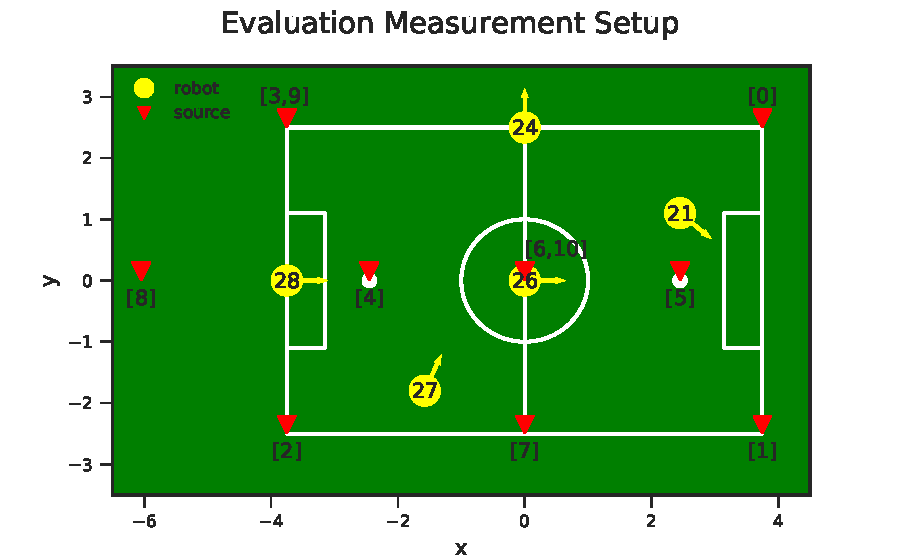
\includegraphics[]{figures/evaluation/setup}
	\caption{Setup of robots and sound source positions for the evaluation measurement.}
    \label{fig:04_setup}
\end{figure}
% -------------------------------------------------------------

\subsection{SNR}
\label{subsec:04_snr}

For the team filter, it the validity a robot result is useful information.
Depending on the uncertainty, the covariance of the incoming result can be adjusted.
Thus, one intuitive hypothesis is assuming the existence of a relation between the
received signal strength and distance to the source.
Taking the measurements of \ref{subsec:04_labMeasurements}, this hypothesis is
investigated by looking at the distance between one robot and the sound source.
According to this distance, it is looked at the \ac{SNR} of one measurement on
one robot proportional to all robots' \acp{SNR} of this measurement.
The \ac{SNR} on a single robot consists of the mean over all microphones' \acp{SNR}.
We can see in \cref{fig:04_snrDistance} that there is no straightforward
link between both values.
Also only taking a frame of size 256 samples into consideration
does not change the result.
% -------------------------------------------------------------
\begin{figure}[ht]
	\centering
		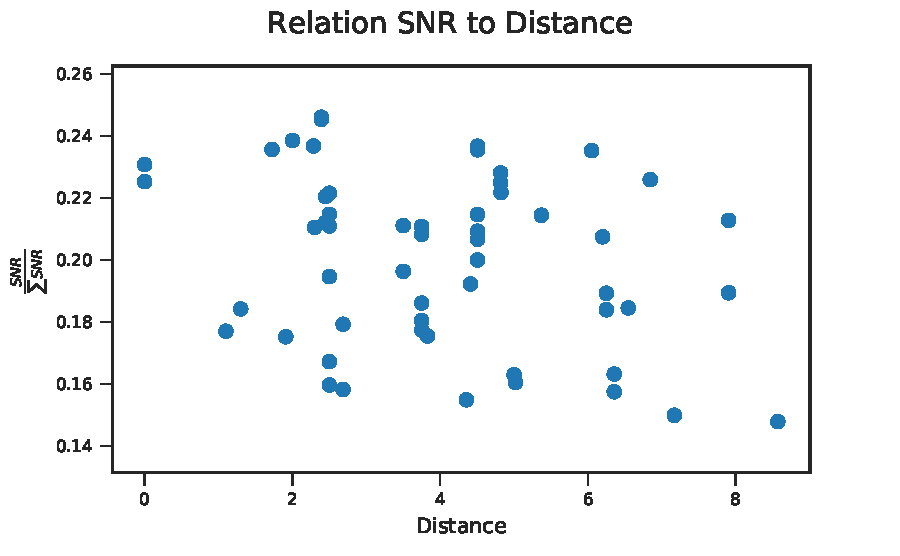
\includegraphics[]{figures/evaluation/snr_scatter}
	\caption{Visualization of relation between SNR and distance.}
    \label{fig:04_snrDistance}
\end{figure}
% -------------------------------------------------------------

Due to the unexpected result, further analysis on the \ac{SNR} values
on individual robots are done.
Therefore, a sine signal with fixed distance to the robot
was recorded from different angles with constant volume.
The main purpose of this measurement is to ensure that the lone channels
are not biased somehow.
Resulting from 14 measurements of a 3\si{\kilo\hertz} sine signal
with are distance of 0.73\si{m}, no tendency could be detected.
Further evaluation is done by determining the channel with the maximum
\ac{SNR} of one measurement. At 85,71\si{\percent} of the cases,
result coincided with the expected channel.
From this, we can say that the general recordings of the microphones
are neither biased nor falsified.

The same investigation is done with the real whistle recordings of the
measurement in \ref{subsec:04_labMeasurements}.
With these measurements only 54,55\si{\percent} of the maximum \acp{SNR}
match with the expected channels.
Consequentially, we must assume that the environmental circumstances
like multi-path propagation and reflection have large influence
on the signal magnitude.

\subsection{PSNR}
\label{subsec:04_psnr}

As referred in \cref{sec:02_gcc}, one characteristic of the \ac{GCC-PHAT}
algorithm is the sharp peak.
In conclusion, one can assume that if no sharp peak can be detected the
delay result of the \ac{GCC} has less informative value.
The validity of this statement is tested by comparing the \ac{PSNR} value
to the error of the direction angle resulting from the \ac{GCC-PHAT} delay.
Two cases of errors are taken into consideration.
In both, the \ac{PSNR} is recorded as high if it exceeds 17,5 whereat the
value ranges from 10,1 to 28,8.

Firstly, each channel pair on one robot is looked at by determining the
smaller error between the actual angle and one of both direction candidates.
If the \ac{PSNR} of the \ac{GCC} is greater than the threshold of 17,5,
the \ac{RMSE} of its result is grouped to the errors with high \ac{PSNR}.
Elsewise it pertains to the errors with low \ac{PSNR}.
This valuation is done with the measurements of \cref{subsec:04_labMeasurements}
and manually set start indexes.
Having 76 correlations assessed with low \ac{PSNR}, the \ac{RMSE} of these
is 35,77\si{\degree}.
Compared to this, the \ac{RMSE} of the remaining 144 measurements
is 15,86\si{\degree}.

To see the impact on a complete robot result, the same is done
with the final errors on single robots.
Here, the \ac{RMSE} of the lower \ac{PSNR} case results in 25,36\si{\degree}
whereat the error of the other case is 14,41\si{\degree}.

From this, one can identify the \ac{PSNR} as valid additional information
for the covariance of a \ac{GCC-PHAT} delay result that enriches the
outcome of a robot direction ray that proceeds into the team filter.

\cleardoublepage
\chapter{Conclusion}
\label{chap:05_conclusion}

The purpose of this work was to find an approach to localize a whistle
signal with a multi-agent system consisting of multiple NAO robots.
Each of these robots have four microphones attached on their head which
record audio signals within a range of 150\si{\hertz} and 12\si{\kilo\hertz}
with a sample rate of 44.1\si{\kilo\hertz}.
Only stationary sound sources and robots were considered in the scope of this
work.
Roughly, the implementation can be divided into three parts.
Of capital importance is the \acf{WSDE} executed by stand-alone robots which
is realized by computing the \ac{TDOA} between the four channels on the robots' head.
Two fundamentally different approaches were evaluated to obtain a stable method
for the delay estimation.
One obtains the \ac{TDOA} by cross-correlating signal samples with standard
\acf{CC} and \acf{GCC-PHAT} algorithms in frequency domain.
The other analyses recorded samples in frequency domain in terms of
a phase of a reference frequency which is described as phase difference method.
% Correct
It was assumed that the start of a signal is most reliable 
To circumvent impact of multi-path propagation and reverberation, 
was examined and is true
Thus, \acf{SSD} approaches were compared with regard to accuracy and computational effort.
Finally, 


% -------------------------------------------------------------
If the observed signal is known as whistle and computational effort is
irrelevant, 
% the evaluation shows that the start detection with the
% existing whistle detection algorithm performs best.
that a rough start detection by the exiting whistle detection
with a large frame size followed by a \ac{ZCR} detection with small
window size.
This is a good trade-off with regard to the computational effort.
% - entropy for large scale start detection\\
% - zcr and energy for smaller scale (because high precision needed)\\


% -------------------------------------------------------------
% \section{TDOA Methods}
% \label{sec:05_methodComparison}

% Phase method: Much faster!

% GCC is more accurate in regard to each robot result -> This is
% important when less robots are used for localization.
% It can be the case when robots are broken / got penalty
% We want each robot result to be as accurate as possible so
% that we can count on each result
% Less robots means, that each wrong direction is weighted more
% and influences the final position significantly.
% -------------------------------------------------------------

% \section{Team Filter}
% \label{sec:05_teamFilter}

% Team filter: more intelligent filtering (e.g. clustering
% intersections for multiple position candidates)

% Future work ___________________________________
% Separation of multiple sounds
% Moving sources, moving robots

% conclusion -> multimodales filtering, expizite ausreißerfilter, include prior knowledge
% of refree position

%############# appendix #################
\cleardoublepage
\renewcommand{\chaptername}{\appendixname} %if name appears in header

\begin{appendix}

	\chapter{Anhang 1}
bla bla bla

bla bla bla



	\cleardoublepage
	\chapter{Anhang 2}
bla bla bla

bla bla bla



\end{appendix}

\cleardoublepage
\phantomsection
\addcontentsline{toc}{chapter}{\protect\numberline{List of Abbreviations}}
\chapter*{List of Abbreviations}
\label{sec:abbreviations}
\markboth{\MakeUppercase{List of Abbreviations}}{\MakeUppercase{List of Abbreviations}}

\begin{acronym}[HSU-HH]
  \acro{CC}[CC]{Cross Correlation}
  \acro{GCC}[GCC]{Generalized Cross Correlation}
  \acro{PHAT}[PHAT]{Phase Transform}
  \acro{GCC-PHAT}[GCC-PHAT]{Generalized Cross Correlation with Phase Transform}
  \acro{HSU}[HSU-HH]{Helmut-Schmidt-University/University of the Federal Armed Forces Hamburg}
  \acro{iFT}[iFT]{inverse Fourier Transform}
  \acro{FFT}[FFT]{Fast Fourier Transform}
  \acro{iFFT}[iFFT]{inverse Fast Fourier Transform}
  \acro{PHAT}[PHAT]{Phase Transform}
  \acro{PDF}[PDF]{Probability Density Function}
  \acro{DFT}[DFT]{Discrete Fourier Transform}
  \acro{STE}[STE]{Short Time Energy}
  \acro{SPL}[SPL]{Standard Platform League}
  \acro{FFTW}[FFTW]{Fastest Fourier Transform in the West}
  \acro{ZCR}[ZCR]{Zero Crossing Rate}
  \acro{TDOA}[TDOA]{Time Difference Of Arrival}
  \acro{SNR}[SNR]{Signal to Noise Ratio}
  \acro{PSNR}[PSNR]{Peak Signal to Noise Ratio}
  \acro{RMSE}[RMSE]{Root Mean Squared Error}
\end{acronym}


%Softwareverzeichnis
\cleardoublepage
\phantomsection
\addcontentsline{toc}{chapter}{\protect\numberline{List of Software}}
\chapter*{List of Software}
\markboth{\MakeUppercase{List of Software}}{\MakeUppercase{List of Software}} 
\label{sec:software}
\begin{table}[htb]
	\centering
		\begin{tabular}{|l|l||l|l|}
		\hline
			\bfseries{Name} & \bfseries{Version} & \bfseries{URL} & \bfseries{Comment}\\
		\hline
		\hline
			Python & 3.7.4 & https://docs.python.org/3/ & \\
		\hline
	... & ... & ... & ... \\
		\hline
		\end{tabular}
	\caption{Verwendete Software.}
	\label{tab:VerwendeteSoftware}
\end{table}

blablabla

\cleardoublepage
%########### Bibliography ##############
\clearpage % to get correct page no. in TOC
\phantomsection
\addcontentsline{toc}{chapter}{\protect\numberline{\bibname}}

\renewcommand{\chaptername}{} %if name appears in header

\renewcommand{\baselinestretch}{1}
\normalsize

% if enabling this command all references of the bib file are listed
% otherwise only the referenced books are listed in Bibliography section
%\nocite{*}

%\bibliographystyle{unsrt}
%\bibliographystyle{alpha}
%\bibliographystyle{ALPHADIN}

\bibliographystyle{IEEEtran} %IEEE Style

% In literature.bib sind die eigentlichen Literaturangaben enthalten
\bibliography{postcontent/literature} % requires file literature.bib


\ifmakeindex
	\cleardoublepage
	\phantomsection
	\addcontentsline{toc}{chapter}{\protect\numberline{Index}}
	% Stichwortverzeichnis endgueltig anzeigen
	\printindex
\fi

\end{document}
